\documentclass{llncs}

\usepackage{makeidx}
\usepackage{amssymb}
\usepackage{listings}
\usepackage{indentfirst}
\usepackage{verbatim}
\usepackage{amsmath, amssymb}
\usepackage{graphicx}
\usepackage{xcolor}
\usepackage{url}
\usepackage{stmaryrd}
\usepackage{xspace}
\usepackage{comment}
\usepackage{wrapfig}
\usepackage{placeins}
\usepackage{tabularx}
\usepackage{ragged2e}


\usepackage [style = gost-numeric, sorting = none] {biblatex}

\addbibresource {main.bib}

\def\transarrow{\xrightarrow}
\newcommand{\setarrow}[1]{\def\transarrow{#1}}

\newcommand{\trule}[2]{\frac{#1}{#2}}
\newcommand{\crule}[3]{\frac{#1}{#2},\;{#3}}
\newcommand{\withenv}[2]{{#1}\vdash{#2}}
\newcommand{\trans}[3]{{#1}\transarrow{#2}{#3}}
\newcommand{\ctrans}[4]{{#1}\transarrow{#2}{#3},\;{#4}}
\newcommand{\llang}[1]{\mbox{\lstinline[mathescape]|#1|}}
\newcommand{\pair}[2]{\inbr{{#1}\mid{#2}}}
\newcommand{\inbr}[1]{\left<{#1}\right>}
\newcommand{\highlight}[1]{\color{red}{#1}}
\newcommand{\ruleno}[1]{\eqno[\scriptsize\textsc{#1}]}
\newcommand{\inmath}[1]{\mbox{$#1$}}
\newcommand{\lfp}[1]{fix_{#1}}
\newcommand{\gfp}[1]{Fix_{#1}}
\newcommand{\vsep}{\vspace{-2mm}}
\newcommand{\supp}[1]{\scriptsize{#1}}
\newcommand{\G}{\mathfrak G}
\newcommand{\sembr}[1]{\llbracket{#1}\rrbracket}
\newcommand{\cd}[1]{\texttt{#1}}
\newcommand{\miniKanren}{miniKanren\xspace}
\newcommand{\ocanren}{OCanren\xspace}
\newcommand{\free}[1]{\boxed{#1}}
\newcommand{\binds}{\;\mapsto\;}
\newcommand{\dbi}[1]{\mbox{\bf{#1}}}

\let\emptyset\varnothing

\lstdefinelanguage{ocanren}{
keywords={fresh, let, in, match, with, when, class, type,
object, method, of, rec, repeat, until, while, not, do, done, as, val, inherit,
new, module, sig, deriving, datatype, struct, if, then, else, open, private, virtual, include, success, failure,
true, false},
sensitive=true,
commentstyle=\small\itshape\ttfamily,
keywordstyle=\ttfamily\underbar,
identifierstyle=\ttfamily,
basewidth={0.5em,0.5em},
columns=fixed,
fontadjust=true,
literate={fun}{{$\lambda$}}1 {->}{{$\to$}}3 {===}{{$\equiv$}}1 {=/=}{{$\not\equiv$}}1 {|>}{{$\triangleright$}}3 {|||}{{$\vee$}}2 {/\\}{{$\wedge$}}2 {^}{{$\uparrow$}}1,
morecomment=[s]{(*}{*)}
}

\lstset{
mathescape=true,
%basicstyle=\small,
identifierstyle=\ttfamily,
keywordstyle=\bfseries,
commentstyle=\scriptsize\rmfamily,
basewidth={0.5em,0.5em},
fontadjust=true,
language=ocanren
}

\usepackage{letltxmacro}
\newcommand*{\SavedLstInline}{}
\LetLtxMacro\SavedLstInline\lstinline
\DeclareRobustCommand*{\lstinline}{%
  \ifmmode
    \let\SavedBGroup\bgroup
    \def\bgroup{%
      \let\bgroup\SavedBGroup
      \hbox\bgroup
    }%
  \fi
  \SavedLstInline
}
\addtolength{\parskip}{-2pt}

\begin{document}
\sloppy
\mainmatter

\title{Typed Relational Conversion}

\author{
  Petr Lozov \and Andrei Vyatkin \and Dmitry Boulytchev
}

\institute{
St.Petersburg State University\\
Universitetski pr., 28, 198504, St.Petersburg, Russia\\
JetBrains Research\\
Universitetskaya emb., 7-9-11, bldg. 5A, 199034, St.Petersburg, Russia}

%\email{lozov.peter@gmail.com}
%\and
%St.Petersburg State University\\
%Universitetski pr., 28, 198504, St.Petersburg, Russia\\
%\email{dewshick@gmail.com}
%\and
%St.Petersburg State University\\
%Universitetski pr., 28, 198504, St.Petersburg, Russia\\
%JetBrains Research\\
%\email{dboulytchev@math.spbu.ru}
%}

\maketitle

\begin{abstract}
We address the problem of transforming typed functional programs into relational form. 
In this form a program can be run in various ``directions'' with some arguments left free, 
making it possible to acquire different behaviors from a single specification. We specify the 
syntax, typing rules and semantics for the source language as well as its relational extension, 
describe the conversion and prove its correctness both in terms of typing and dynamic semantics. 
We also discuss the limitations of our approach, present the implementation of the conversion for 
the subset of OCaml and evaluate it on a number of realistic examples.
\end{abstract}

\section{Introduction}
\label{sec:intro}

Algebraic data types (ADT) is an important tool in functional programming which delivers a way to represent flexible and easy to manipulate data structures.
To inspect the contents of ADT values a generic construct~--- \emph{pattern matching}~--- is used. Pattern matching can be considered as a generalization of
conventional conditional control-flow construct ``\lstinline|if .. then .. else|'' and in principle can be decomposed into a nested hierarchy of those; from
this standpoint the problem of pattern matching implementation can be considered trivial. However, some decompositions are obviously better than others. We
repeat here an example from~\cite{maranget2008} to demonstrate this difference (see Fig.~\ref{fig:match-example}). Here we match a triple of boolean
values $x$, $y$, and $z$ against four pattern (Fig.~\ref{fig:matching-example1}; we use \textsc{OCaml}~\cite{ocaml} as reference language). The na\"{i}ve
implementation of this example is shown on Fig.~\ref{fig:matching-example2}; however if we decide to match $y$ first the result becomes much
better (Fig.~\ref{fig:matching-example3}).

\begin{figure}[ht]
\begin{subfigure}[t]{0.2\linewidth}
\centering
\begin{lstlisting}
match x, y, z with
| _, F, T -> 1
| F, T, _ -> 2
| _, _, F -> 3
| _, _, T -> 4
\end{lstlisting}
\vskip18.5mm
\caption{Pattern matching}
\label{fig:matching-example1}
\end{subfigure}
\hspace{0.5cm}
\begin{subfigure}[t]{0.26\linewidth}
\centering
\begin{lstlisting}
if x then
  if y then
    if z then 4 else 3
  else
    if z then 1 else 3
else
  if y then 2
  else
    if z then 1 else 3
\end{lstlisting}
\caption{A correct but non-optimal\\\phantom{(b)~}implementation}
\label{fig:matching-example2}
\end{subfigure}
\hspace{0.5cm}
\begin{subfigure}[t]{0.33\linewidth}
\centering
\begin{lstlisting}
if y then
  if x then
    if z then 4 else 3
  else 2
else
  if z then 1 else 3
\end{lstlisting}
\vskip13.5mm
\caption{Optimal implementation}
\label{fig:matching-example3}
\end{subfigure}
\caption{Pattern matching implementation example} 
\label{fig:match-example}
\end{figure}

\begin{comment}
\begin{figure}[ht]
\begin{minipage}[b]{0.3\linewidth}
\centering
\label{fig:figure1}
\end{minipage}
\hspace{0.5cm}
\begin{minipage}[b]{0.3\linewidth}
\centering
\begin{lstlisting}
switch x with 
| true -> 
    switch y with 
    | true -> 
       switch z with 
       | true -> 4
       | _ -> 3
    | _ -> 
      switch z with 
      | true -> 1
      | _ -> 3 
| _ -> 
   switch y with 
   | true -> 2 
   | _ -> if z then 1 else 3
\end{lstlisting}
\end{minipage}
\hspace{0.5cm}
\begin{minipage}[b]{0.3\linewidth}
\centering
\end{minipage}
\end{figure}
\end{comment}


%clasification 1
Although semantics of pattern matching can be given as a sequence of srutinee's sub expression comparisons (Figure~\ref{fig:matchpatts}) effective compilers don't follow
this approach. One can either optimise runtime cost by minimizing amount of checks performed or static cost by minimizing the size of generated code. \emph{Decision trees}~\cite{?}
are good for the first criteria, because they check every subexpression not more than once. \emph{Backtracking automata} are rather compact but in some cases can perform
repeated checks.

%clasification 2
\emph{For strict languages} checking sub-expressions of scrutinee in any order is allowed. \emph{For lazy languages} pattern matching should evaluate only those sub-expressions which are
necessary for performing pattern matching. If not careful pattern matching can change the termination behavior of the program. In general lazy languages setup more constraints on pattern matching and because of that allow lesser set of heuristics. Decision trees and backtracking automata can be used for compilation both  strict and lazy languages.

%clasification 3
The matching compilers for strict languages can work in \emph{direct} or \emph{indirect} styles. The first ones return efficient code immediately. In the second style to
construct final answer some post processing is required. It can vary from easy simplifications to complicated supercompilation techniques~\cite{sestoft1996}. The main
drawback of indirect style is that the size of intermediate data structures can be exponentially large.

% about lazy languages
A few approaches for checking sub-expressions in lazy languages has been proposed. In ~\cite{augustsson1985} simple left-to-right order of subexpression checking was proposed and was proved that it doesn't affect termination. The backtracking automaton being built has a form of a DAG to reduce code size. A few refinements has been added by~\cite{wadler1987} as a part of textbook~\cite{peytonjones1987} about implementing lazy functional languages. The implementation from this book is being used in the current version of GHC~\cite{ghc}. \cite{laville1991} models values in lazy languages
using \emph{partial terms}, although it doesn't scale to types with infinite constructor sets (like integers). The approach doesn't test all subexpressions from left to right as~\cite{augustsson1985} but aims to not perform unnecessary check by constructing \emph{lazy automaton}. 
%In~\cite{suarez1993} the similar approach is extended by special treatment of overlapping patterns.

% about decision trees
Pattern matching for lazy languages has been compiled also to decision trees~\cite{maranget1992} and later (\cite{maranget1994}) into
\emph{decision DAGs} which allow in some cases to make code smaller.

Minimizing the size of decision tree is known to be NP-hard~\cite{baudinet1985tree}, and as a rule various heuristics are applied during compilation, for example, the number of nodes,
the length of the longest path, the average length of all paths. The paper~\cite{Scott2000WhenDM} performs experimental evaluation of nine heuristics on the base of for strict language Standard ML of New Jersey.

%about automata
The inefficiency of backtracking automaton has been
improved in~\cite{maranget2001}. The approach utilizes matrix representation for pattern matching. It splits the current matrix according to constructors in the
first column and reduces the task to compiling matrices with less rows. The technique is indirect, in the end a few optimizations are performed by introducing
special \emph{exit} nodes to the compiled representation. No preprocessing is required for this scheme: or-pattern receives a special treatment during compilation process.
The approach from this paper is used in the current implementation of the \textsc{OCaml} compiler.

Previous approach uses first column to split the matrix. In~\cite{maranget2008} the \emph{necessity} heuristic has been introduced which recommends which column should be
used to perform the split. Good decision trees which are constructed in this work can perform better on corner cases than~\cite{maranget2001}, but for practical cases the
difference is insignificant.


While existing approaches deliver appropriate solutions for certain forms of pattern matching construct, they have to be extended in an \emph{ad hoc} manner each time
the syntax and semantics of pattern matching construct changes. For example, besides a simple conventional form of pattern matching there is a number of extensions
(guards~\cite{?}, disjunctive patterns~\cite{?}, non-linear patterns~\cite{mcbride1969symbol}, active patterns~\cite{activepatterns}, pattern matching for polymorphic variants~\cite{Garrigue98} and generalized
algebraic datatypes~\cite{?}) which require a separate customized algorithms to be developed.

\begin{comment}
\begin{minipage}[b]{0.5\textwidth}
There are a few different approaches for compiling pattern mathcing. For example, \textsc{GHC}~\cite{?} uses that presented in an influential paper~\cite{Jones1987},
implementation of pattern matching in \textsc{OCaml} is currently based on~\cite{maranget2001} although \cite{maranget2008} reports a slight improvements
of generated code efficiency. 
\end{minipage}
\end{comment}

We present an approach to pattern matching implementation based on application of relational programming~\cite{TRS,WillThesis} and, in particular, relational interpreters~\cite{unified}
and relational conversion~\cite{lozov2017}. Our approach is based on relational representation of the top-level source language semantics of pattern matching on the one hand, and
the semantics of intermediate-level implementation language on the other. We formulate the condition for a correct and complete implementation of pattern matching and use it to
construct a top-level goal which represents a search procedure for all correct and complete implementations. We also present a number of techniques which makes it possible to come up with an
\emph{optimal} solution as well as optimizations to improve the performance of the search. Our implementation\footnote{\url{https://github.com/kakadu/pat-match}} makes use of
\textsc{OCanren}\footnote{\url{https://github.com/JetBrains-Research/OCanren}}~--- a typed implementation of \textsc{miniKanren} for \textsc{OCaml}~\cite{OCanren},
and \textsc{noCanren}\footnote{\url{https://github.com/Lozov-Petr/noCanren}}~--- a convertor from the subset of plain \textsc{OCaml} into \textsc{OCanren}~\cite{lozov2017}.
An evaluation, performed for a set of benchmarks taken from other papers, initially has shown a good performance of our synthesizer. However, being aware of some pitfalls of
our approach, we came up with a set of counterexamples, on which it did not provide any results in observable time, so we do not consider the problem completely solved.
We also started a work on mechanized formalization\footnote{\url{https://github.com/dboulytchev/Coq-matching-workout}}, written in \textsc{Coq}~\cite{Coq}, to
make the justification of out approach more solid and easier to verify, but this formalization is not yet complete. 

 

\documentclass[submission,copyright,creativecommons]{eptcs}
%\providecommand{\event}{SOS 2007} % Name of the event you are submitting to

\usepackage{breakurl}             % Not needed if you use pdflatex only.
\usepackage{underscore}           % Only needed if you use pdflatex.
\usepackage{amssymb}
\usepackage{listings}
\usepackage{indentfirst}
\usepackage{verbatim}
\usepackage{amsmath, amsthm, amssymb}
\usepackage{graphicx}
\usepackage{url}
\usepackage{hyperref}
\usepackage{xspace}

\lstdefinelanguage{ocaml}{
keywords={fresh, let, begin, end, in, match, type, and, fun, function, try, with, when, class, 
object, method, of, rec, repeat, until, while, not, do, done, as, val, inherit, 
new, module, sig, deriving, datatype, struct, if, then, else, open, private, virtual},
sensitive=true,
%basicstyle=\small,
commentstyle=\small\itshape\ttfamily,
keywordstyle=\ttfamily\underbar,
identifierstyle=\ttfamily,
basewidth={0.5em,0.5em},
columns=fixed,
fontadjust=true,
literate={->}{{$\to\;\;$}}3 {===}{{$\equiv$}}3 {=/=}{{$\not\equiv$}}3,
morecomment=[s]{(*}{*)}
}

\lstset{
%basicstyle=\small,
mathescape=true,
identifierstyle=\ttfamily,
keywordstyle=\bfseries,
commentstyle=\scriptsize\rmfamily,
basewidth={0.5em,0.5em},
fontadjust=true,
%escapechar=~,
language=ocaml
}

\sloppy

\newcommand{\miniKanren}{\texttt{miniKanren}\xspace}

\title{Typed Embedding of a Relational Language in OCaml}
\author{Dmitry Kosarev
\institute{Saint Petersburg State University\\ Saint Petersburg, Russia}
\email{Dmitrii.Kosarev@protonmail.ch}
\and
Dmitry Boulytchev
\institute{Saint Petersburg State University\\ Saint Petersburg, Russia}
\email{dboulytchev@math.spbu.ru}
}
\def\titlerunning{Typed Embedding of a Relational Language in OCaml}
\def\authorrunning{Dmitry Kosarev, Dmitry Boulytchev}
\begin{document}
\maketitle

\begin{abstract}
We present an implementation of the relational programming language \miniKanren as a set 
of combinators and syntax extension for OCaml. The key feature of our approach is 
\emph{polymorphic unification}, which can be used to unify data structures of almost 
arbitrary types. In addition we provide a useful generic programming pattern to 
systematically develop relational specifications in a typed manner, and address 
the problem of relational and functional code integration.
\end{abstract}

\section{Introduction}
\label{sec:intro}

Algebraic data types (ADT) is an important tool in functional programming which delivers a way to represent flexible and easy to manipulate data structures.
To inspect the contents of ADT values a generic construct~--- \emph{pattern matching}~--- is used. Pattern matching can be considered as a generalization of
conventional conditional control-flow construct ``\lstinline|if .. then .. else|'' and in principle can be decomposed into a nested hierarchy of those; from
this standpoint the problem of pattern matching implementation can be considered trivial. However, some decompositions are obviously better than others. We
repeat here an example from~\cite{maranget2008} to demonstrate this difference (see Fig.~\ref{fig:match-example}). Here we match a triple of boolean
values $x$, $y$, and $z$ against four pattern (Fig.~\ref{fig:matching-example1}; we use \textsc{OCaml}~\cite{ocaml} as reference language). The na\"{i}ve
implementation of this example is shown on Fig.~\ref{fig:matching-example2}; however if we decide to match $y$ first the result becomes much
better (Fig.~\ref{fig:matching-example3}).

\begin{figure}[ht]
\begin{subfigure}[t]{0.2\linewidth}
\centering
\begin{lstlisting}
match x, y, z with
| _, F, T -> 1
| F, T, _ -> 2
| _, _, F -> 3
| _, _, T -> 4
\end{lstlisting}
\vskip18.5mm
\caption{Pattern matching}
\label{fig:matching-example1}
\end{subfigure}
\hspace{0.5cm}
\begin{subfigure}[t]{0.26\linewidth}
\centering
\begin{lstlisting}
if x then
  if y then
    if z then 4 else 3
  else
    if z then 1 else 3
else
  if y then 2
  else
    if z then 1 else 3
\end{lstlisting}
\caption{A correct but non-optimal\\\phantom{(b)~}implementation}
\label{fig:matching-example2}
\end{subfigure}
\hspace{0.5cm}
\begin{subfigure}[t]{0.33\linewidth}
\centering
\begin{lstlisting}
if y then
  if x then
    if z then 4 else 3
  else 2
else
  if z then 1 else 3
\end{lstlisting}
\vskip13.5mm
\caption{Optimal implementation}
\label{fig:matching-example3}
\end{subfigure}
\caption{Pattern matching implementation example} 
\label{fig:match-example}
\end{figure}

\begin{comment}
\begin{figure}[ht]
\begin{minipage}[b]{0.3\linewidth}
\centering
\label{fig:figure1}
\end{minipage}
\hspace{0.5cm}
\begin{minipage}[b]{0.3\linewidth}
\centering
\begin{lstlisting}
switch x with 
| true -> 
    switch y with 
    | true -> 
       switch z with 
       | true -> 4
       | _ -> 3
    | _ -> 
      switch z with 
      | true -> 1
      | _ -> 3 
| _ -> 
   switch y with 
   | true -> 2 
   | _ -> if z then 1 else 3
\end{lstlisting}
\end{minipage}
\hspace{0.5cm}
\begin{minipage}[b]{0.3\linewidth}
\centering
\end{minipage}
\end{figure}
\end{comment}


%clasification 1
Although semantics of pattern matching can be given as a sequence of srutinee's sub expression comparisons (Figure~\ref{fig:matchpatts}) effective compilers don't follow
this approach. One can either optimise runtime cost by minimizing amount of checks performed or static cost by minimizing the size of generated code. \emph{Decision trees}~\cite{?}
are good for the first criteria, because they check every subexpression not more than once. \emph{Backtracking automata} are rather compact but in some cases can perform
repeated checks.

%clasification 2
\emph{For strict languages} checking sub-expressions of scrutinee in any order is allowed. \emph{For lazy languages} pattern matching should evaluate only those sub-expressions which are
necessary for performing pattern matching. If not careful pattern matching can change the termination behavior of the program. In general lazy languages setup more constraints on pattern matching and because of that allow lesser set of heuristics. Decision trees and backtracking automata can be used for compilation both  strict and lazy languages.

%clasification 3
The matching compilers for strict languages can work in \emph{direct} or \emph{indirect} styles. The first ones return efficient code immediately. In the second style to
construct final answer some post processing is required. It can vary from easy simplifications to complicated supercompilation techniques~\cite{sestoft1996}. The main
drawback of indirect style is that the size of intermediate data structures can be exponentially large.

% about lazy languages
A few approaches for checking sub-expressions in lazy languages has been proposed. In ~\cite{augustsson1985} simple left-to-right order of subexpression checking was proposed and was proved that it doesn't affect termination. The backtracking automaton being built has a form of a DAG to reduce code size. A few refinements has been added by~\cite{wadler1987} as a part of textbook~\cite{peytonjones1987} about implementing lazy functional languages. The implementation from this book is being used in the current version of GHC~\cite{ghc}. \cite{laville1991} models values in lazy languages
using \emph{partial terms}, although it doesn't scale to types with infinite constructor sets (like integers). The approach doesn't test all subexpressions from left to right as~\cite{augustsson1985} but aims to not perform unnecessary check by constructing \emph{lazy automaton}. 
%In~\cite{suarez1993} the similar approach is extended by special treatment of overlapping patterns.

% about decision trees
Pattern matching for lazy languages has been compiled also to decision trees~\cite{maranget1992} and later (\cite{maranget1994}) into
\emph{decision DAGs} which allow in some cases to make code smaller.

Minimizing the size of decision tree is known to be NP-hard~\cite{baudinet1985tree}, and as a rule various heuristics are applied during compilation, for example, the number of nodes,
the length of the longest path, the average length of all paths. The paper~\cite{Scott2000WhenDM} performs experimental evaluation of nine heuristics on the base of for strict language Standard ML of New Jersey.

%about automata
The inefficiency of backtracking automaton has been
improved in~\cite{maranget2001}. The approach utilizes matrix representation for pattern matching. It splits the current matrix according to constructors in the
first column and reduces the task to compiling matrices with less rows. The technique is indirect, in the end a few optimizations are performed by introducing
special \emph{exit} nodes to the compiled representation. No preprocessing is required for this scheme: or-pattern receives a special treatment during compilation process.
The approach from this paper is used in the current implementation of the \textsc{OCaml} compiler.

Previous approach uses first column to split the matrix. In~\cite{maranget2008} the \emph{necessity} heuristic has been introduced which recommends which column should be
used to perform the split. Good decision trees which are constructed in this work can perform better on corner cases than~\cite{maranget2001}, but for practical cases the
difference is insignificant.


While existing approaches deliver appropriate solutions for certain forms of pattern matching construct, they have to be extended in an \emph{ad hoc} manner each time
the syntax and semantics of pattern matching construct changes. For example, besides a simple conventional form of pattern matching there is a number of extensions
(guards~\cite{?}, disjunctive patterns~\cite{?}, non-linear patterns~\cite{mcbride1969symbol}, active patterns~\cite{activepatterns}, pattern matching for polymorphic variants~\cite{Garrigue98} and generalized
algebraic datatypes~\cite{?}) which require a separate customized algorithms to be developed.

\begin{comment}
\begin{minipage}[b]{0.5\textwidth}
There are a few different approaches for compiling pattern mathcing. For example, \textsc{GHC}~\cite{?} uses that presented in an influential paper~\cite{Jones1987},
implementation of pattern matching in \textsc{OCaml} is currently based on~\cite{maranget2001} although \cite{maranget2008} reports a slight improvements
of generated code efficiency. 
\end{minipage}
\end{comment}

We present an approach to pattern matching implementation based on application of relational programming~\cite{TRS,WillThesis} and, in particular, relational interpreters~\cite{unified}
and relational conversion~\cite{lozov2017}. Our approach is based on relational representation of the top-level source language semantics of pattern matching on the one hand, and
the semantics of intermediate-level implementation language on the other. We formulate the condition for a correct and complete implementation of pattern matching and use it to
construct a top-level goal which represents a search procedure for all correct and complete implementations. We also present a number of techniques which makes it possible to come up with an
\emph{optimal} solution as well as optimizations to improve the performance of the search. Our implementation\footnote{\url{https://github.com/kakadu/pat-match}} makes use of
\textsc{OCanren}\footnote{\url{https://github.com/JetBrains-Research/OCanren}}~--- a typed implementation of \textsc{miniKanren} for \textsc{OCaml}~\cite{OCanren},
and \textsc{noCanren}\footnote{\url{https://github.com/Lozov-Petr/noCanren}}~--- a convertor from the subset of plain \textsc{OCaml} into \textsc{OCanren}~\cite{lozov2017}.
An evaluation, performed for a set of benchmarks taken from other papers, initially has shown a good performance of our synthesizer. However, being aware of some pitfalls of
our approach, we came up with a set of counterexamples, on which it did not provide any results in observable time, so we do not consider the problem completely solved.
We also started a work on mechanized formalization\footnote{\url{https://github.com/dboulytchev/Coq-matching-workout}}, written in \textsc{Coq}~\cite{Coq}, to
make the justification of out approach more solid and easier to verify, but this formalization is not yet complete. 

 

\section{Streams, States, and Goals}
\label{sec:goals}

This section describes a top-level framework for our implementation. Despite it contains
nothing more, then a reiteration of the original implementation~\cite{MicroKanren, CKanren} 
in OCaml, we still need some notions to be properly established.

\miniKanren is organized as a set of combinators, designated to describe a search for
the solution of a certain \emph{goal}. The search itself is implemented using a
backtracking lazy stream monad:

\begin{lstlisting}
   type 'a stream

   val mplus : 'a stream -> 'a stream -> 'a stream
   val bind  : 'a stream -> ('a -> 'b stream) -> 'b stream
\end{lstlisting}

Monadic primitives describe the shape of the search, and their implementations may 
vary in concrete \miniKanren versions.

An essential component of the implementation is a bundle of the following types

\begin{lstlisting}
   type env         = $\dots$
   type subst       = $\dots$
   type constraints = $\dots$

   type state = env * subst * constraints
\end{lstlisting}

Type \lstinline{state} describes a point in a lazily constructed search tree: type \lstinline{env} corresponds 
to an \emph{environment}, which contains some supplementary information (in particular, environment is needed to
correctly allocate fresh variables), type \lstinline{subst} describes a substitution, which keeps current bindings 
for some logical variables, and, finally, type \lstinline{constraints} represents disequality constraints, 
which have to be respected. In a simplest case \lstinline{env} is just a counter for the number of next free
variable, \lstinline{subst} is a map-like structure and \lstinline{constraints} is a list of substitutions. In our
case environment contains some extra information to make it possible to identify variables in constant time.

The next cornerstone is the \emph{goal} type, which is considered as a transformer of a state into 
lazy stream of state:

\begin{lstlisting}
   type goal = state -> state stream
\end{lstlisting}

In terms of search, a goal nondeterministically performs one step of the search: for a given
node in a search tree it produces its immediate descendants.

Next to last, there is a number of predefined combinators:

\begin{lstlisting}
   val (&&&)      : goal -> goal -> goal
   val (|||)      : goal -> goal -> goal
   val call_fresh : ($v$ -> goal) -> goal
   ....
\end{lstlisting}

Conjunction \lstinline{&&&} combines the results of its argument goals using \lstinline{bind}, 
disjunction \lstinline{|||} concatenates the results using \lstinline{mplus}, abstraction
primitive \lstinline{call_fresh} takes an abstracted goal and applies it to a freshly created
variable. Type $v$ in latest case designated the type for a fresh variable, which we leave
abstract for now. These conbinators serves as bricks for implementation of conventional 
\miniKanren constructions and syntax extensions (\lstinline{conde}, \lstinline{fresh} etc.)

Finally, there are two primitive goal constructors:

\begin{lstlisting}
   val (===) : $t$ -> $t$ -> goal
   val (=/=) : $t$ -> $t$ -> goal
\end{lstlisting}

The first one is unification, while the other~--- disequality constraint. Here we, again, left 
the type of terms $t$ abstract; it will be instantiated later.

In the implementation of \miniKanren both these goals are implemented using unification~\cite{CKanren}; this
is true for us as well. However, due to a drastic difference in host languages the implementation of
efficient polymorphic unification itself leads to a number of tricks with typing and data representation,
non-existing in the original version.


\section{Polymorphic Unification}
\label{sec:unification}

We consider it rather natural to employ polymorphic unification in a language already equipped
with polymorphic comparison~--- a convenient, but somewhat disputable\footnote{See, for example,
\url{https://blogs.janestreet.com/the-perils-of-polymorphic-compare}} feature. Like polymorphic comparison,
polymorphic unification performs a traversal of values, exploiting intrinsic knowledge of their runtime
representation. The undeniable benefits of this solution are, first, that in order to perform unification
for user types no ``boilerplate'' code is needed, and, second, that this approach seems to deliver the
most efficient implementation. On the other hand, all the pitfalls of polymorphic comparison are inherited as
well; in particular, polymorphic unification loops for cyclic data structures and does not work for functional
values. Since we generally do not expect any reasonable outcome in these cases, the only remaining problem is that
the compiler is incapable of providing any assistance in identifying and avoiding these cases. Another drawback is that
the implementation of polymorphic unification relies on the runtime representation of values and has to be fixed
every time the representation changes.  Finally, as it is written in an unsafe manner using the \lstinline{Obj} interface,
it has to be carefully developed and tested.

An important difference between polymorphic comparison and unification is that the former only inspects its operands,
while the results of unification are recorded in a substitution (a mapping from logical variables to terms), which
later is used to reify answers. So, generally speaking, we have to show that no ill-typed
terms are constructed as a result. Overall, this property seems to be maintained vacuously, since the very
nature of (syntactic) unification is to detect whether some things can be considered equal. Nevertheless there are
different type systems and different unification implementations; in addition \emph{equal things} can be
\emph{differently typed}, so we provide here a correctness justification for a well-defined abstract case, and will
reuse this conclusion for various concrete cases.

First, we consider three alphabets:

$$
\begin{array}{rcl}
  \tau,\dots&-&\mbox{types}\\
  x^\tau,\dots&-&\mbox{typed logic variables}\\
  C_k^{\tau_1\times\tau_2\times\dots\times\tau_k\to\tau} (k\ge 0),\dots&-&\mbox{typed constructors}
\end{array}
$$

The set of all well-formed typed terms is defined by mutual induction for all types:

$$
t^\tau=x^\tau\mid C_k^{\tau_1\times\tau_2\times\dots\times\tau_k\to\tau}(t^{\tau_1},\,t^{\tau_2},\,\dots,\,t^{\tau_k})
$$

For simplicity from now on we abbreviate the notation $C_k^{\tau_1\times\tau_2\times\dots\times\tau_k\to\tau}(t^{\tau_1},\,t^{\tau_2},\,\dots,\,t^{\tau_k})$ into
$C_k^\tau(t^{\tau_1},\,t^{\tau_2},\,\dots,\,t^{\tau_k})$, keeping in mind that for any concrete constructor and for all its occurrences
in arbitrary terms all its subterms in corresponding positions agree in types.

\begin{comment}
We need also to define the notion of a subterm  $t^\tau[p]$ of a term $t^\tau$ at given position $p$:

$$
\begin{array}{rcl}
 p=\epsilon\mid\{1, 2, 3,\dots\}\bullet p&-&\mbox{the set of positions}\\
 t^\tau[\epsilon]=t^\tau&-&\mbox{base case}\\
 C_k^\tau(t_1^{\tau_1},\,t_2^{\tau_2},\dots,\,t_k^{\tau_k})[i\bullet p]=t_i^{\tau_i}[p], 1\le i \le k&-&\mbox{inductive case}
\end{array}
$$
\end{comment}

In this formulation we do not consider any structure over the set of types besides type equality, and we assume all terms are explicitly
attributed by their types at runtime. We employ this property to implement a unification algorithm in regular OCaml, using some
representation for terms and types:

\begin{lstlisting}[mathescape=true]
    val unify : term -> term -> subst option -> subst option
\end{lstlisting}

\noindent where ``\lstinline{term}'' stands for the type, representing typed terms, ``\lstinline{subst}'' stands for the type of
substitution (a partial mapping from logic variables to terms). Unification can fail (hence ``\lstinline{option}'' in the result type),
is performed in the context of existing substitution (hence ``\lstinline{subst}'' in the third argument) and can be
chained (hence ``\lstinline{option}'' in the third argument).

We use exactly the same unification algorithm with triangular substitution as in the reference implementation~\cite{MicroKanren}. We
omit here some not-so-important details (like ``occurs check'') and refrain from discussing the nature and properties of the algorithm
itself (an excellent description, including a certified correctness proof, can be found in~\cite{Kumar}).

The following snippet presents the implementation:

\begin{lstlisting}[mathescape=true,numbers=left,numberstyle=\small,stepnumber=1,numbersep=-5pt]
    let rec unify $t_1^\tau$ $t_2^\tau$ $subst$ =
      let rec walk $s$ $t^\tau$ =
        match $t^\tau$ with
        | $x^\tau$ when $x^\tau\in dom(s)$ -> $\;\;$walk $s$ $(s\;\;x^\tau)$
        | _ -> $t^\tau$
      in
      match $subst$ with
      | None -> None
      | Some $s$ ->
          match walk $s$ $t_1^\tau$, walk $s$ $t_2^\tau$ with
          | $x_1^\tau$, $x_2^\tau$ when $x_1^\tau$ = $x_2^\tau$ -> $subst$
          | $x_1^\tau$, $q_2^\tau$ -> Some ($s\;[x_1^\tau \gets q_2^\tau]$)
          | $q_1^\tau$, $x_2^\tau$ -> Some ($s\;[x_2^\tau \gets q_1^\tau]$)
          | $C^\tau(t_1^{\tau_1},\dots,t_k^{\tau_k})$, $C^\tau(p_1^{\tau_1},\dots,p_k^{\tau_k})$ ->
              unify $t_k^{\tau_k}$ $p_k^{\tau_k}$(.. (unify $t_1^{\tau_1}$ $p_1^{\tau_1}$ $subst$)$..$)
          | $\_$, $\_$ -> None
\end{lstlisting}

We remind the reader that all superscripts correspond to type attributes, which we consider here as
parts of values being manipulated. For example, line 1 means that we apply \lstinline{unify}
to terms $t_1$ and $t_2$, and expect their types to be equal $\tau$. We assume that
at the top level unification is always applied to some terms of the same type, and that any
substitution can only be acquired from the empty one by a sequence of unifications.

We are going to show that under these assumptions all type attributes are superfluous~--- they
do not affect the execution of \lstinline{unify} and can be removed. Note that the only place where we
were incapable of providing an explicit type attribute was in the line 4, where the result of
substitution application was returned. However, we can prove by induction that any substitution
respects the following property: if a substitution $s$ is defined for a variable $x^\tau$,
then $s\;\;x^\tau$ is attributed with the type $\tau$ (and, consequently, \lstinline{walk $s$ $t^\tau$} always
returns a term of type $\tau$).

Indeed, this property vacuously holds for the empty substitution. Let $s$ be some substitution, for which the
property holds. In the line 11 we return an unchanged substitution; in line 10 we perform two calls~---
\lstinline{walk $s$ $t_1^\tau$} and \lstinline{walk $s$ $t_2^\tau$} and match their results. However,
by our induction hypothesis these results are again attributed by the type $\tau$, which justifies the
pattern matching. In line 11 we return the substitution unchanged, in lines 12 and 13 we extend the
existing substitution, but preserve the property of interest. Finally, in line 15 we chain a few
applications of \lstinline{unify}; note that, again, all these calls are performed for terms of equal
types, starting from a substitution possessing the property of interest. A simple induction on the
chain length completes the proof.

So, type attributes are inessential~--- they are never analyzed and never restrict pattern matching; hence,
they can be erased completely. 
We can notice now that for the representation of terms we can use OCaml's native runtime representation. 
It can not be done, however, using regular OCaml~--- we have to utilize the low-level, unsafe interface \lstinline{Obj}. 
Note also, we need some way to identify the occurrences of logical variables inside the terms (in the original \miniKanren
implementation the ambiguity between variable and non-variable datum representation is resolved by a convention~--- a luxury 
we cannot afford).  We postpone the discussion of this subject until the next section.


%the correctness our of implementation is based on
%the following convention about logical variables: the representation of a logical variable $x^\tau$ must
%correspond to a representation of some value of type $\tau$. This, in turn, makes it somewhat problematic
%to detect a variable occurrence in a term. We postpone the discussion of this subject until Section~\ref{sec:injection}.

We call our implementation \emph{polymorphic}, since at the top level it is defined as

\begin{lstlisting}
   val unify : $\alpha$ -> $\alpha$ -> subst option -> subst option
\end{lstlisting}

The type of substitution is not polymorphic, which means that the compiler completely loses track
of types for values stored in a substitution. These types are recovered later during the reification-of-answers phase (see Section~\ref{sec:reification}).
Outside the unification the compiler maintains typing, which means that all terms, subterms, and variables agree in their types
in all contexts.

\section{Logic Variables and Injection}
\label{sec:injection}

Unification, considered in Section~\ref{sec:unification}, works for values of any types. However, it
is too generic to be used directly. As long as we use it to unify closed terms, it's ok (but rather meaningless); 
however, for terms with free variables the situation becomes more complicated. Indeed, as we've seen in the
previous section, a variable $x^\tau$ must have a runtime representation of some value of type $\tau$. As different
types may not have any values in common, if we wish to unify arbitrary types, we would need to specify the 
ground type for each logical variable explicitly, which would overthrow our implementation into a non-polymorphic 
realm with no type inference.

In this part we consider two approaches to safely handling typed terms, while preserving polymorphism and
type inference. The first is rather easy to develop and implement; unfortunately, the implementation demonstrates 
poor performance for a number of important applications. In order to fix this defficiency, we develop more 
elaborated technique, which nevertheless reuses some components from the previous one. In Section~\ref{sec:evaluation}
we present the results of performance evaluation for both approaches and compare them to that of original 
implementation.

\subsection{Tagged Logical Values}

The first natural solution is to restrict the unification to logic values only. We introduce the following polymorphic
type $[\alpha]$\footnote{In concrete syntax called ``$\alpha\;$\lstinline{logic}''}, which corresponds to a type, injected into
logic domain:

\begin{lstlisting}
   type $[\alpha]$ = Var of int | Value of $\alpha$
\end{lstlisting}

Note, this type cannot be disclosed to a end-user, since the only possible way to create a logic variable should 
still be by using ``\lstinline{fresh}'' construct.

Informally speaking, any value of type $[\alpha]$ is either a value of type $\alpha$, or a free
logic variable. Now, we may redefine the signature of abstraction, unification and disequality primitives in the
following manner

\begin{lstlisting}
   val call_fresh : ($[\alpha]$ -> goal) -> goal

   val (===)      : $[\alpha]$ -> $[\alpha]$ -> goal
   val (=/=)      : $[\alpha]$ -> $[\alpha]$ -> goal
\end{lstlisting}

Both unification and disequality constraint would still use the same polymorphic unification; their external, visible type,
however, is restricted to logical types only.

Apart from variables, other logical values can be obtained by injection; conversely, sometimes logical value can be projected to 
a regular one. We supply two basic functions\footnote{In concrete syntax called ``\lstinline{inj}'' and ``\lstinline{prj}''.}
for these purposes

\begin{lstlisting}[mathescape=true]
   val ($\uparrow_\forall$) : $\alpha$ -> $[\alpha]$ 
   val ($\downarrow_\forall$) : $[\alpha]$ -> $\alpha$

   let ($\uparrow_\forall$) x = Value x
   let ($\downarrow_\forall$) = function Value x -> x | _ -> failwith $\mbox{``not a value''}$
\end{lstlisting}

which can be used to perform a \emph{shallow} injection/projection. As expected, the injection is total, while the projection is partial. 
Using these functions and type-specific functors, which can be derived automatically using a number of existing frameworks for 
generic programming, one can easily provide injection and projection for user-defined datatypes.

We consider user-defined list type as an example:

\begin{lstlisting}[mathescape=true]
   type ($\alpha$, $\beta$) list$_f$ = Nil | Cons of $\alpha$ * $\beta$
   
   type $\alpha$ list = ($\alpha$, $\alpha$ list) list$_f$
   type $\alpha$ list$_l$ = $[$($[\alpha]$, $\alpha$ list$_l$) list$]$

   let rec $\uparrow_{\mbox{\texttt{list}}}$ l = $\uparrow$($fmap_{\mbox{\texttt{list}}_f}$ ($\uparrow_\forall$) $\uparrow_{\mbox{\texttt{list}}}$ l) 
   let rec $\downarrow_{\mbox{\texttt{list}}}$ l = $fmap_{\mbox{\texttt{list}}_f}$ ($\downarrow_\forall$) $\downarrow_{\mbox{\texttt{list}}}$ ($\downarrow_\forall$ l)
\end{lstlisting}

Here ``\lstinline{list$_f$}'' is a custom functor for lists. We provide two specialized versions~--- ``\lstinline{list}'', 
which corresponds to regular, non-logic lists, and ``\lstinline{list}$_l$'', which corresponds to logical lists with logical elements. 
Using a single type-specific function \lstinline{$fmap_{\mbox{\texttt{list}}_f}$}, we easily build both injection of type 

\begin{lstlisting}
   $\alpha$ list -> $\alpha$ list$_l$
\end{lstlisting} 

and projection of type 

\begin{lstlisting}
   $\alpha$ list$_l$ -> $\alpha$ list
\end{lstlisting}

Generally speaking, we can always implement injection/projection for arbitrary regular type, represented as a fixpoint of a functor~\cite{ALaCarte}, 
using only $\uparrow_\forall$, $\downarrow_\forall$ and a small set of datatype-generic combinators.

We now can address the problem of variable identification during polymorphic unification. As we do not know the types, we cannot discriminate logical 
variables by their tags only and, thus, cannot simply use pattern matching. In our implementation we perform variable test 
as follows:

\begin{itemize}
\item in environment, we additionally keep some unique boxed value~--- \emph{anchor}~--- created by \lstinline{run} at the moment of initial
state generation; the anchor is inherited unchanged in all derived environments during the search session;
\item in each variable we additionally save the anchor, inherited from the environment, in which the variable was created;
\item inside a unification, in order to check, if we deal with a variable, we test the conjuction of the following properties:

  \begin{enumerate}
    \item the scrutenee is boxed; 
    \item the scrutenee's tag and layout correspond to those for variables;
    \item the scrutenee's anchor and current environment anchor addresses are equal.
  \end{enumerate}
\end{itemize}

Taking into account, that the state type is abstract at the user level, we guarantee, that only those variables, which were
created during current run session would pass the test, since the pointer to anchor is unique among all pointers to a boxed values 
and could not be disclosed elsewhere but in the variable creation primitive.

The only thing to describe now is the implementation of the refinement stage. The refinement is represented by the following 
function:

\begin{lstlisting}
   val refine : state -> $[\alpha]$ -> $[\alpha]$ 
\end{lstlisting}

This function takes a state and a logical value and recursively substitutes all logical variables in that value w.r.t. 
the substitution in the state until no occurrences of bound variables left. Since in our implementation the type of substitution is
not polymorphic, \lstinline{refine} is also implemented in an unsafe manner. However, it is easy to see, that \lstinline{refine} 
does not produce ill-typed terms. Indeed, all original types of variables are preserved in a substitution; unification does not 
change unified terms, so all terms, bound in a substitution, are well-typed. Hence, \lstinline{refine} always substitutes
some subterm in a well-typed term with another term of the same type, which preserves well-typedness.

In addition to performing substitutions, \lstinline{refine} also reifies disequality constrains. Reification 
attaches to each free variable in a refined term a list of \emph{refined} terms, describing the disequality constraints for that
free variable. Note, disequality can be established only for equally-typed terms, which justifies type-safety of reification. 
Note also, additional care has to be taken to avoid infinite looping, since refinement and reification are
mutually recursive, and refinement of a variable can be potentially invoked from itself due to a chain of disequality 
constraints.

After refinement, the content of a logical value can be inspected via the following function:

\begin{lstlisting}
   val destruct : $[\alpha]$ -> [`Var of int * $[\alpha]$ list | `Value of $\alpha$]
\end{lstlisting}

Constructor \lstinline{`Var} corresponds to a free variable with unique integer identifier and a list of terms, 
representing all disequality constraints for this variable. These terms are refined as well.

\subsection{Tagless Logical Values and Type Bookeeping}

The solution, presented in the previous subsection, suffers from the following defficiency: in order to perform unification,
we inject terms into logic domain, making them as twice as large. As a result, this implementation loses the original one in 
terms of performance in many important applications, which compromises the very idea of using OCaml as a host language.

Here we develop an advanced version, which eliminates this penalty. As a first step, let's try to eliminate the tagging with
a drastic measure:

\begin{lstlisting}
   type $[\alpha]$ = $\alpha$
\end{lstlisting}

What consequences would this have? Of course, we would not be able to create logical variables in a conventional way. However, 
we still could have a separate type for variables

\begin{lstlisting}
   type var = Var of int * anchor
\end{lstlisting}

and use \emph{the same} variable test procedure. As the type $[\alpha]$ is abstract, this modification does not change the interface. 
As we reuse the variable test, polymorphic unification can continue work \emph{almost} correctly. The problem is that
now it can introduce the occurrences of free logic variables in non-logical, tagless, data structures. These free logic variables 
do not get in the way of unification itself (since it can handle them properly, thanks to the variable test), but they can not
be disclosed to the outer world as is.

Our idea is to use this generally unsound representation for all internal actions, and perform tagging only during the refinement
stage. However, this scenario raises the following question: what whould the type of \lstinline{refine} be? It can not be simply

\begin{lstlisting}
   val refine : state -> $[\alpha]$ -> $[\alpha]$
\end{lstlisting}

anymore since $[\alpha]$ now equals $\alpha$. We \emph{want}, however, it be something like

\begin{lstlisting}
   val refine : state -> $[\alpha]$ -> $(\mbox{``tagged'' }[\alpha])$
\end{lstlisting}

If $\alpha$ is not a parametric type, we can simply test, if the value is a variable, and if yes, tag it with constructor \lstinline{Var};
otherwise we tag it with \lstinline{Value}, and we're done. This trick, however, would not work for parametric types. Consider, for example, 
the refinement of a value of type \lstinline{$[[$int$]$ list$]$}. The (hypotetical) approach being described would return a value of
type \lstinline{$(\mbox{``tagged'' }[[$int$]$ list$])$}, i.e. tagged only on the top level; we need to repeat the procedure
recursively. In other words, we need the following (meta) type for the refinement primitive:

\begin{lstlisting}
   val refine : state -> $[\alpha]$ -> $\mbox{(``tagged''} [\beta])$
\end{lstlisting}

where $\beta$ is the result of tagging $\alpha$.

These considerations can be boiled down to the following concrete implementation. 

First, we roll back to the initial definition of $[\alpha]$~--- it will play role of our ``tagged'' type.
We introduce a new, two-parametric type\footnote{In concrete syntax $(\alpha,\;\beta)\;$\lstinline{injected}.}

\begin{lstlisting}
   type $\{\alpha,\;\beta\}$ = $\alpha$
\end{lstlisting}

Of course, this type is kept abstract at the end-user level. Informally speaking, type $\{\alpha,\;\beta\}$ designates the
injection of tagless type $\alpha$ into tagged type $\beta$; the value itself is kept in the tagless form, but
tagged type can be used during the refinement stage as a constraint, which would allow to refine tagless
representation only to a feasible tagged one.

We introduce the following primivites for the type $\{\alpha,\;\beta\}$:

\begin{lstlisting}
   val lift : $\alpha$ -> $\{\alpha,\;\alpha\}$
   val inj  : $\{\alpha,\;\beta\}$ -> $\{\alpha,\;[\beta]\}$

   let lift x = x
   let inj  x = x
\end{lstlisting}

The function \lstinline{lift} puts a value into the ``bookeeping injection'' domain for the first time, while
\lstinline{inj} plays the role of injection itself. Their composition is analogous to what was 
called ``$\uparrow_\forall$'' in the previous implementation:

\begin{lstlisting}
   val $\uparrow_\forall$ : $\alpha$ -> $\{\alpha,\;[\alpha]\}$
   let $\uparrow_\forall$ x = lift x |> inj
\end{lstlisting}

In order to deal with parametric types, we can again utilize generic programming. To handle the types with
one parameter, we introduce the following functor:

\begin{lstlisting}
   module FMap (T : sig type $\alpha$ t val fmap : ($\alpha$ -> $\beta$) -> $\alpha$ t -> $\beta$ t end) :      
     sig 
       val distrib : $\{\alpha,\;\beta\}$ T.t -> $\{\alpha$ T.t, $\beta$ T.t$\}$ 
     end =
     struct
       let distrib x = x
     end
\end{lstlisting}

Note, that we do not use function ``\lstinline{T.fmap}'' in the implementation; however, first, we need an inhabitant of
corresponding type to make sure we indeed deal with a functor, and next, we actually will use it in the 
implementation of type-specific refinement, see below).

In order to handle two-, three-, etc. parametric types we need higher-kinded polymorphism, which is
not supported in a direct form in OCaml. So, unfortunately, we need to introduce a separate
functors for the types with two-, three- etc. parameters; existing works on higher-kinded
polymorphism in OCaml~\cite{HKinded} require the similar scaffolding to be erected as a bootstrap step.

Given the functor(s) of described shape, we can use it in the following manner:

\begin{lstlisting}
   module FOption = FMap 
     (struct 
        type $\alpha$ t = $\alpha$ option 
        let fmap = $fmap_{\mbox{\texttt{option}}}$ 
      end
     )

   val some : $\{\alpha, \beta\}$ -> $\{\alpha\mbox{\texttt{ option}},\;\beta\mbox{\texttt{ option}}\}$
   val none : unit  -> $\{\alpha\mbox{\texttt{ option}},\;\beta\mbox{\texttt{ option}}\}$
   
   let some x  = FOption.distrib (Some x) |> inj
   let none () = FOption.distrib None     |> inj
\end{lstlisting}

In other words, we can in a very systematic manner define \emph{logic representatives} for all constructors
of types of interest. These representatives can be used in the relational code, providing a well-bookept
typing~--- for each logical type we would be able to reconstruct its original, tagless preimage. 

With the new implementation, the types for ``basic'' goal constructors have to be adjusted:

\begin{lstlisting}
   val (===) : $\{\alpha,\;[\beta]\}$ -> $\{\alpha,\;[\beta]\}$ -> goal
   val (=/=) : $\{\alpha,\;[\beta]\}$ -> $\{\alpha,\;[\beta]\}$ -> goal
\end{lstlisting}

As always, we require both arguments of unification and disequalify constraint to be of the same type; in addition
we require the ``injected'' part of the type to be logic.

During the refinement stage the bindings for ``integersting'' variables, reconstructed using the final
substitution, have to be properly tagged. This process as well is implemented in a datatype-generic manner:
fisrt, we have refiners for primitive types:

\begin{lstlisting}
   val refine$_{\mbox{\texttt{int}}}$ : helper -> $\{$int,$[$int$]\}$ -> $[$int$]$
   val refine$_{\mbox{\texttt{string}}}$ : helper -> $\{$string,$[$string$]\}$ -> $[$string$]$
   ...  
\end{lstlisting}

and, then, we add the refiner to the output signature in all \lstinline{FMap}-like functors:

\begin{lstlisting}
   val refine: (helper -> $\{\alpha,\;\beta\}$ -> $\beta$) -> helper -> $\{\alpha$ T.t, $[\beta$ T.t$]$ as $\gamma\}$ -> $\gamma$
\end{lstlisting}

Note, since now \lstinline{refine} is type-specific and, hence, constructed at the user-level, we refrain from passing 
it a state (otherwise it would be a user's responsibility to refine variables only in appropriate states). 
Instead, we wrap all state-specific functionality in abstract \lstinline{helper} data type, which encapsulates
all functionality, needed for \lstinline{refine} to work properly.

\section{Refinement and Top-Level Primitives}
\label{refinement}

We do not make final search states accessible for an end-user; instead we provide
a set of top-level combinators, which should be used to surround relational code
and perform refinement in a transparent manner. Note, from pragmatic
standpoint only variables, supplied as arguments for the top-level goal, have
to be refined (the original \miniKanren implementation follows the same convention).

The toplevel primitive in our implementation is \lstinline{run}, which takes three
arguments. The exact type of \lstinline{run} is rather complex and non-instructive, 
so we better describe the typical form of its application:

\begin{lstlisting}[mathescape=true]
   run $\overline{n}$ (fun $l_1\dots l_n$ -> $\;\;G$) (fun $a_1\dots a_n$ -> $\;\;H$)
\end{lstlisting}

Here $\overline{n}$ stands for \emph{numeral}, which describes the number of
parameters for two other arguments of \lstinline{run}, \mbox{$l_1\dots l_n$}~---
free logical variables, $G$~--- a goal (which can make use of \mbox{$l_1\dots l_n$}), 
\mbox{$a_1\dots a_n$}~--- refined answers for \mbox{$l_1\dots l_n$}, respectively, and, 
finally, $H$~--- a \emph{handler} (which can make use of \mbox{$a_1\dots a_n$}). 

The types of \mbox{$l_1\dots l_n$} are inferred from $G$ and always have a form

\begin{lstlisting}
   $\{\alpha,\;[\beta]\}$
\end{lstlisting}

since the types of variables can be constrained only in unification or disequality constraints.

The types of \mbox{$a_1\dots a_n$} are inferred from types of \mbox{$l_1\dots l_n$} and
have the form

\begin{lstlisting}
   $(\alpha,\;\beta)$ refined stream
\end{lstlisting}

where the type \lstinline{refined}, in turn, is

\begin{lstlisting}
   type ($\alpha$, $\beta$) refined = $<\;$prj : $\alpha$; refine : (helper -> $\{\alpha,\;\beta\}$ -> $\beta$) -> $\beta>$
\end{lstlisting}

Two methods of this type can be used to perform two different styles of refinement: first, a value without
free variables can be returned as is (method \lstinline{prj} does this: it checks, that in the value of
interest no free variables occur, and raises an exception otherwise). If the value contains free
variables, it has to be properly injected into the logic domain~--- this is what \lstinline{refine} stands
for. It takes as an argument a type-specific tagging function, constructed using generic
primitives, described in the previous section.

In other words, user-defined handler takes streams of refined answers for all variables, supplied to the top-level 
goal. All streams $a_i$ contains coherent elements, so they all have the same length and $n$-th elements of all 
streams correspond to the $n$-th answer, produced by the goal $G$.

There are a few predefined numerals for one, two, etc. arguments (called, by tradition, 
\lstinline{q}, \lstinline{qr}, \lstinline{qrs} etc.), and a successor function, which 
can be applied to existing numeral to increment the number of expected arguments. The
implementation technique generally follows~\cite{Unparsing, DoWeNeed}.

\section{Examples}
\label{sec:examples}

In this section we present some examples of relational specification, written with the aid of our library.
Besides \miniKanren combinators themselves, our implementation contains two syntax extensions~--- one
for \lstinline{fresh} construct and another for \emph{inverse-$\eta$-delay}~\cite{MicroKanren}, which is
sometimes necessary to delay recursive calls in order to prevent infinite looping. In addition we included a
small relational library of data structures like lists, numbers, booleans, etc. This library is written
completely on the user level using techniques described in Section~\ref{sec:injection} with no utilization
of any unsafe features. The examples given below illustrate the usage of all these elements as well.

\subsection{List Concatenation and Reversing}

List concatenation and reversing are usually the first relational programs considered, and we do not wish
to deviate from this tradition. We've already considered the implementation of \lstinline{append$^o$} in
original \miniKanren in Section~\ref{sec:demo}. In our case, the implementation looks familiar:

\begin{lstlisting}
   let rec append$^o$ x y xy =
     (x === nil ()) &&& (y === xy) |||
     (fresh (h t)
       (x === h % t) &&&
       (fresh (ty)
         (h % ty === xy) &&& (append$^o$ t y ty)
       )
     )

   let rec revers$^o$ a b =
     conde [
       (a === nil ()) &&& (b === nil ());
       (fresh (h t)
         (a === h % t) &&&
         (fresh (a')
           (append$^o$ a' !< h b) &&& (revers$^o$ t a')
         )
       )
     ]
\end{lstlisting}

Here we make use of our implementation of relational lists, which provides convenient shortcuts for
standard functional primitives:

\begin{itemize}
  \item ``\lstinline{nil ()}'' corresponds to ``\lstinline{[]}'';
  \item ``\lstinline{h % t}'' corresponds to ``\lstinline{h::t}'';
  \item ``\lstinline{a %< (b %< (c !< d))}'' corresponds to ``\lstinline{[a; b; c; d]}''.
\end{itemize}

In our implementation the basic \miniKanren primitive ``\lstinline{conde}'' is implemented as a
disjunction of a list of goals, not as a built-in syntax construct. We also make use of explicit
conjunction and disjunction infix operators instead of nested bracketed structures which, we
believe, would look too foreign here.

\subsection{Relational Sorting and Permutations}

For the next example we take list sorting; specifically, we present a sorting for lists of natural numbers
in Peano form since our library already contains built-in support for them. However our example can be
easily extended for arbitrary (but linearly ordered) types.

List sorting can be implemented in \miniKanren in a variety of ways~--- virtually any existing algorithm can
be rewritten relationally. We, however, try to be as declarative as possible to demonstrate the
advantages of the relational approach. From this standpoint, we can claim that the sorted version of an empty list is an
empty list, and the sorted version of a non-empty list is its smallest element, concatenated with a sorted
version of the list containing all its remaining elements.

The following snippet literally implements this definition:

\begin{lstlisting}
   let rec sort$^o$ x y =
     conde [
       (x === nil ()) &&& (y === nil ());
       fresh (s xs xs')
         (y === s % xs')
         (sort$^o$ xs xs')
         (smallest$^o$ x s xs)
     ]
\end{lstlisting}

The meaning of the expression ``\lstinline{smallest$^o$ x s xs}'' is ``\lstinline{s} is the smallest element of a (non-empty) list \lstinline{x}, and \lstinline{xs} is the
list of all its remaining elements''. Now, \lstinline{smallest$^o$} can be implemented using a case analysis (note, ``\lstinline{l}'' here is a non-empty list):

\begin{lstlisting}
   let rec smallest$^o$ l s l' =
     conde [
       (l === s % nil ()) &&& (l' === nil ());
       fresh (h t s' t' max)
         (l' === max % t') &&&
         (l === h % t) &&&
         (minmax$^o$ h s' s max) &&&
         (smallest$^o$ t s' t')
     ]
\end{lstlisting}

Finally, we implement a relational minimum-maximum calculation
primitive:

\begin{lstlisting}
   let minmax$^o$ a b min max =
     conde [
       (min === a) &&& (max === b) &&& (le$^o$ a b);
       (max === a) &&& (min === b) &&& (gt$^o$ a b)
     ]
\end{lstlisting}

Here ``\lstinline{le$^o$}'' and ``\lstinline{gt$^o$}'' are built-in comparison goals for natural numbers in Peano form.

Having relational \lstinline{sort$^o$}, we can implement sorting for regular integer lists:

\begin{lstlisting}
   let sort l =
     run q (sort$^o$ @@ inj_nat_list l)
           (fun qs -> from_nat_list @@ (Stream.hd qs)#prj)
\end{lstlisting}

Here \lstinline{Stream.hd} is a function which takes a head from a lazy stream of answers,
\lstinline{inj_nat_list}~--- injection from regular integer lists into logical lists of logical Peano numbers,
\lstinline{from_nat_list}~--- projection from lists of Peano numbers to lists of integers.

It is interesting, that since \lstinline{sort$^o$} is
relational, it can be used to calculate the list of all \emph{permutations}
for a given list. Indeed, sorting each permutation results in the same list.
So, the problem of finding all permutations can be relationally reformulated into
the problem of finding all lists which are converted by sorting into the given one:

\begin{lstlisting}
let perm l = map (fun a -> a#prj |> from_nat_list) @@
  run q (fun q -> fresh (r)
                    (sort$^o$ (inj_nat_list l) r)
                    (sort$^o$ q r)
        )
        (Stream.take ~n:(fact @@ length l))
\end{lstlisting}

Note, for sorting the original list we used exactly the same primitive. Note also,
we requested exactly \lstinline{fact @@ length l} answers; requesting more
would result in an infinite search for non-existing answers.

\subsection{Type Inference for STLC}

Our final example is a type inferencer for Simply Typed Lambda Calculus~\cite{Lambda}. The problem and
solution themselves are rather textbook examples again~\cite{TRS, WillThesis}; however, with this example
we show once again the utilization of generic programming techniques we described in Section~\ref{sec:injection}.
As a supplementary generic programming library here we used object-oriented generic transformers\footnote{\url{https://github.com/dboulytchev/GT}};
we presume, however, that any other framework could equally be used.

We first describe the type of lambda terms and their logic representation:

\begin{lstlisting}
   module Term =
     struct
       module T =
         struct
           @type ('varname, 'self) t =
           | V   of 'varname
           | App of 'self    * 'self
           | Abs of 'varname * 'self
           with gmap

           let fmap f g x = gmap(t) f g x
         end

     include T
     include FMap2(T)

     let v   s   = inj @@ distrib @@ V s
     let app x y = inj @@ distrib @@ App (x, y)
     let abs x y = inj @@ distrib @@ Abs (x, y)
   end
\end{lstlisting}

Now we have to repeat the work for the type of simple types:

\begin{lstlisting}
   module Type =
     struct
       module T =
         struct
           @type ('a, 'b) t =
           | P   of 'a
           | Arr of 'b * 'b
           with gmap

          let fmap f g x = gmap(t) f g x
        end

       include T
       include FMap2(T)

       let p   s   = inj @@ distrib @@ P s
       let arr x y = inj @@ distrib @@ Arr (x, y)
     end
\end{lstlisting}

Note, the ``relational'' part is trivial, boilerplate and short (and could even be generated
using a more advanced framework).

The relational type inferencer itself rather resembles the original implementation. The only
difference (besides the syntax) is that instead of data constructors we use their logic
counterparts:

\begin{lstlisting}
   let rec lookup$^o$ a g t =
     fresh (a' t' tl)
       (g === (inj_pair a' t') % tl) &&&
       (conde [
         (a' === a) &&& (t' === t);
         (a' =/= a) &&& (lookup$^o$ a tl t)
       ])

   let infer$^o$ expr typ =
     let rec infer$^o$ gamma expr typ =
       conde [
         fresh (x)
           (expr === v x) &&&
           (lookupo x gamma typ);
         fresh (m n t)
           (expr === app m n) &&&
           (infer$^o$ gamma m (arr t typ)) &&&
           (infer$^o$ gamma n t);
         fresh (x l t t')
           (expr === abs x l) &&&
           (typ  === arr t t') &&&
           (infer$^o$ ((inj_pair x t) % gamma) l t')
       ]
     in
     infer$^o$ (nil()) expr typ
\end{lstlisting}

\section{Conclusion}

We presented a strongly-typed implementation of \miniKanren for OCaml. Our implementation
passes all tests written for \miniKanren (including those for disequality constraints);
in addition we implemented many interesting relational programs known from
the literature. We claim that our implementation can be used both as a convenient
relational DSL for OCaml and an experimental framework for future research in the area of
relational programming.

%We also want to express our gratitude to William Byrd, who infected us with relational programming,
%and for the extra time he sacrificed as both our tutor and friend.


\begin{thebibliography}{99}
\bibitem{TRS}
Daniel P. Friedman, William E.Byrd, Oleg Kiselyov. The Reasoned Schemer. The MIT
Press, 2005.

\bibitem{MicroKanren}
Jason Hemann, Daniel P. Friedman. $\mu$Kanren: A Minimal Core for Relational Programming //
Proceedings of the 2013 Workshop on Scheme and Functional Programming (Scheme '13).

\bibitem{CKanren}
Claire E. Alvis, Jeremiah J. Willcock, Kyle M. Carter, William E. Byrd, Daniel P. Friedman.
cKanren: miniKanren with Constraints // 
Proceedings of the 2011 Workshop on Scheme and Functional Programming (Scheme '11).

\bibitem{Untagged}
William E. Byrd, Eric Holk, Daniel P. Friedman.
miniKanren, Live and Untagged: Quine Generation via Relational Interpreters (Programming Pearl) //
Proceedings of the 2012 Workshop on Scheme and Functional Programming (Scheme '12).

\bibitem{Implicits}
Leo White, Fr\'ed\'eric Bour, Jeremy Yallop. 
Modular Implicits // Workshop on ML, 2014, arXiv:1512.01438.

\bibitem{Unparsing}
Olivier Danvy.
Functional Unparsing // Journal of Functional Programming, Vol.~8, Issue~6, November 1998.

\bibitem{DoWeNeed}
Daniel Fridlender, Mia Indrika.
Do we need dependent types? // Journal of Functional Programming, Vol.~10, Issue~4, July 2000.

\bibitem{DGP}
Jeremy Gibbons. Datatype-generic Programming //
Proceedings of the 2006 International Conference on Datatype-generic Programming.

\bibitem{Deriving}
Jeremy Yallop. 
Practical Generic Programming in OCaml // Proceedings of 2007 Workshop on ML.

\bibitem{InstantGenerics}
Manuel M. T. Chakravarty, Gabriel C. Ditu, Roman Leshchinskiy. 
Instant Generics: Fast and Easy. \url{http://www.cse.unsw.edu.au/~chak/papers/CDL09.html}, 2009.

\bibitem{ALaCarte}
Wouter Swierstra. Data Types \'a la Carte  // Journal of Functional Programming, Vol.~18, Issue~4, 2008.

\bibitem{Kumar}
Ramana Kumar. Mechanising Aspects of miniKanren in HOL. Bachelor Thesis, The Australian National University, 2010.

\bibitem{Unification}
Franz Baader, Wayne Snyder. Unification theory. In John Alan Robinsonand Andrei Voronkov, editors, 
Handbook of Automated Reasoning. Elsevier and MIT Press, 2001.

\bibitem{triangular}
David C Bender, Lindsey Kuper, William E Byrd, Daniel P Friedman. 
Efficient Representations for Triangular Substitutions: a Comparison in miniKanren. Indiana University, 2009.

\end{thebibliography}

\end{document}


\begin{figure*}[t]
\[
\begin{array}{cccll}
  &\mathcal{C} & = & \{C_i^{k_i}\} & \mbox{constructors with arities} \\
  &\mathcal{T}_X & = & X \cup \{C_i^{k_i} (t_1, \dots, t_{k_i}) \mid t_j\in\mathcal{T}_X\} & \mbox{terms over the set of variables $X$} \\
  &\mathcal{D} & = & \mathcal{T}_\emptyset & \mbox{ground terms}\\
  &\mathcal{X} & = & \{ x, y, z, \dots \} & \mbox{syntactic variables} \\
  &\mathcal{A} & = & \{ \alpha, \beta, \gamma, \dots \} & \mbox{semantic variables} \\
  &\mathcal{R} & = & \{ R_i^{k_i}\} &\mbox{relational symbols with arities} \\[2mm]
  &\mathcal{G} & = & \mathcal{T_X}\equiv\mathcal{T_X}   &  \mbox{unification} \\
  &            &   & \mathcal{G}\wedge\mathcal{G}     & \mbox{conjunction} \\
  &            &   & \mathcal{G}\vee\mathcal{G}       &\mbox{disjunction} \\
  &            &   & \mbox{\lstinline|fresh|}\;\mathcal{X}\;.\;\mathcal{G} & \mbox{fresh variable introduction} \\
  &            &   & R_i^{k_i} (t_1,\dots,t_{k_i}),\;t_j\in\mathcal{T_X} & \mbox{relational symbol invocation} \\[2mm]
  \phantom{XXXXXXXXXXXXXXX}&\mathcal{S} & = & \{R_i^{k_i} = \lambda\;x_1^i\dots x_{k_i}^i\,.\, g_i;\}\; g & \mbox{specification}
  %      ^
  %      |
  %  this ugly hack is due to non-working \centering
\end{array}
\]
\caption{The syntax of the source language}
\label{syntax}
\end{figure*}

\begin{figure}[t]
\centering
\[
\begin{array}{c}
  \mathcal{FV}\,(x)=\{x\}\\
  \mathcal{FV}\,(C_i^{k_i}\,(t_1,\dots,t_k))=\bigcup\mathcal{FV}\,(t_i)\\[2mm]
  \mathcal{FV}\,(t_1\equiv t_2)=\mathcal{FV}\,(t_1)\cup\mathcal{FV}\,(t_2)\\
  \mathcal{FV}\,(g_1\wedge g_2)=\mathcal{FV}\,(g_1)\cup\mathcal{FV}\,(g_2)\\
  \mathcal{FV}\,(g_1\vee g_2)=\mathcal{FV}\,(g_1)\cup\mathcal{FV}\,(g_2)\\
  \mathcal{FV}\,(\mbox{\lstinline|fresh|}\;x\;.\;g)=\mathcal{FV}\,(g)\setminus\{x\}\\
  \mathcal{FV}\,(R_i^{k_i}\,(t_1,\dots,t_k))=\bigcup\mathcal{FV}\,(t_i)
\end{array}
\]
\caption{Free variables in terms and goals}
\label{free}
\end{figure}

\section{The Language}
\label{language}
 
In this section we introduce the syntax of the language we use throughout the paper, describe the informal semantics and give some examples.

The syntax of the language is shown on Figure~\ref{syntax}. First, we fix a set of constructors $\mathcal{C}$ with known arities and consider
a set of terms $\mathcal{T}_X$ with constructors as functional symbols and variables from $X$. We parameterize this set with an alphabet of
variables, since in the semantic description we will need \emph{two} kinds of variables. The first kind, \emph{syntactic} variables, is denoted
by $\mathcal{X}$. We also consider an alphabet of \emph{relational symbols} $\mathcal{R}$ which are used to name relational definitions.
The central syntactic category in the language is \emph{goal}. In our case there are five types of goals: \emph{unification} of terms,
conjunction and disjunction of goals, fresh variable introduction and invocation of some relational definition. Thus, unification is used
as a constraint, and multiple constraints can be combined using conjunction, disjunction and recursion. For the sake of brevity we
abbreviate immediately nested ``\lstinline|fresh|'' constructs into the one, writing ``\lstinline|fresh $x$ $y$ $\dots$ . $g$|'' instead of
``\lstinline|fresh $x$ . fresh $y$ . $\dots$ $g$|''. The final syntactic category is \emph{specification} $\mathcal{S}$. It consists of a set
of relational definitions and a top-level goal. A top-level goal represents a search procedure which returns a stream of substitutions for
the free variables of the goal. The definition for set of free variables for both terms and goals is given on Figure~\ref{free}; as ``\lstinline|fresh|''
is the sole binding construct the definition is rather trivial. The language we defined is first-order, as goals can not be passed as parameters,
returned or constructed at runtime.

We now informally describe how relational search works. As we said, a goal represents a search procedure. This procedure takes a \emph{state} as input and returns a
stream of states; a state (among other information) contains a substitution which maps semantic variables into terms over semantic variables. Then the five types of
scenarios are possible (depending on the type of the goal):

\begin{itemize}
\item Unification ``\lstinline|$t_1$ === $t_2$|'' unifies terms $t_1$ and $t_2$ in the context of the substitution in the current state. If terms are unifiable,
  then their MGU is integrated into the substitution, and one-element stream is returned; otherwise the result is an empty stream.
\item Conjunction ``\lstinline|$g_1$ /\ $g_2$|'' applies $g_1$ to the current state and then applies $g_2$ to the each element of the result, concatenating
  the streams.
\item Disjunction ``\lstinline|$g_1$ \/ $g_2$|'' applies both its goals to the current state independently and then concatenates the results.
\item Fresh construct ``\lstinline|fresh $x$ . $g$|'' allocates a new semantic variable $\alpha$, substitutes all free occurrences of $x$ in $g$ with $\alpha$, and
  runs the goal.
\item Invocation ``$\lstinline|$R_i^{k_i}$ ($t_1$,...,$t_{k_i}$)|$'' finds a definition for the relational symbol $R_i^{k_i}=\lambda x_1\dots x_{k_i}\,.\,g_i$, substitutes
  all free occurrences of formal parameter $x_j$ in $g_i$ with term $t_j$ (for all $j$) and runs the goal in the current state.
\end{itemize}

We stipulate that the top-level goal is preceded by an implicit ``\lstinline|fresh|'' construct, which binds all its free variables, and that the final substitutions
for these variables constitute the result of the goal evaluation.

Conjunction and disjunction form a monadic~\cite{Monads} interface with conjunction playing role of ``bind'' and disjunction~--- of ``mplus''. In this description
we swept a lot of important details under the carpet~--- for example, in actual implementations the components of disjunction are not evaluated in isolation, but
both disjuncts are being evaluated incrementally with the control passing from one disjunct to another (\emph{interleaving}); instead streams the implementation
can be based on ``ferns''~\cite{BottomAvoiding} to defer divergent computations, etc. 

As an example consider the following specification:

\begin{lstlisting}
  append$^o$ = fun x y xy .
    ((x === Nil) /\ (xy === y)) \/
    (fresh h t ty .
       (x  === Cons (h, t))  /\
       (xy === Cons (h, ty)) /\
       (append$^o$ y t ty)
    );
  revers$^o$ = fun x y .
    ((x === Nil) /\ (y === Nil)) \/
    (fresh h t t' .
       (x === Cons (h, t)) /\
       (append$^o$ t' (Cons (h, Nil)) y) /\
       (revers$^o$ t t') 
    );
  revers$^o$ x x
\end{lstlisting}

Here we defined\footnote{We respect here a conventional tradition for \textsc{miniKanren} programming to superscript all relational names with ``$^o$''.}
two relational symbols~--- ``\lstinline|append$^o$|'' and ``\lstinline|revers$^o$|'',~--- and specified a top-level goal ``\lstinline|revers$^o$ x x|''.
The symbol ``\lstinline|append$^o$|'' defines a relational concatenation of lists~--- it takes three arguments and performs a case analysis on the first one. If the
first one is an empty list (``\lstinline|Nil|''), then the second and the third arguments are unified. Otherwise the first argument is deconstructed into a head ``\lstinline|h|''
and a tail ``\lstinline|t|'', and the tail is concatenated with the second argument using a recursive call to ``\lstinline|append$^o$|'' and additional variable ``\lstinline|ty|'', which
represents the concatenation of ``\lstinline|t|'' and ``\lstinline|y|''. Finally, we unify ``\lstinline|Cons (h, ty)|'' with ``\lstinline|xy|'' to form a final constraint. Similarly,
``\lstinline|revers$^o$|'' defines relational list reversing. The top-level goal represents a search procedure for all lists ``\lstinline|x|'', which are stable under reversing, i.e.
represent palindromes. Running it results in an infinite stream of substitutions:

\begin{lstlisting}
   $\alpha\;\mapsto\;$ Nil
   $\alpha\;\mapsto\;$ Cons ($\beta_0$, Nil)
   $\alpha\;\mapsto\;$ Cons ($\beta_0$, Cons ($\beta_0$, Nil))
   $\alpha\;\mapsto\;$ Cons ($\beta_0$, Cons ($\beta_1$, Cons ($\beta_0$, Nil)))
   $\dots$
\end{lstlisting}

where ``$\alpha$''~--- a \emph{semantic} variable, corresponding to ``\lstinline|x|'', ``$\beta_i$''~--- free semantics variables.

The syntax described above can be formalized in \textsc{Coq} in a natural way using inductive data types. We have made a few non-essential simplifications and modifications for the sake of convenience.
Specifically, we restrict the arities of constructors to be either zero or two:

\begin{lstlisting}[language=Coq,basicstyle=\footnotesize]
   Inductive term : Set :=
   | Var : var -> term
   | Cst : con_name -> term
   | Con : con_name -> term -> term -> term.
\end{lstlisting}

Here ``\lstinline[language=Coq]{var}'' and ``\lstinline[language=Coq]{con_name}''~--- the types representing variables and constructor names, whose definitions we omitted for the sake of brevity.
Similarly, we restrict relations to always have exactly one argument:

\begin{lstlisting}[language=Coq,basicstyle=\footnotesize]
   Definition rel : Set := term -> goal.
\end{lstlisting}

These restrictions do not make the language less expressive in any way since we can represent a sequence of terms as a list using constructors \lstinline|Nil$^0$| and \lstinline|Cons$^2$|.

We also introduce one additional type of goals~--- \emph{failure}~--- for deliberately unsuccessful computation (empty stream). As a result, the definition of goals looks as follows:

\begin{lstlisting}[language=Coq,basicstyle=\footnotesize]
   Inductive goal : Set :=
   | Fail   : goal
   | Unify  : term -> term -> goal
   | Disj   : goal -> goal -> goal
   | Conj   : goal -> goal -> goal
   | Fresh  : (var -> goal) -> goal
   | Invoke : rel_name -> term -> goal.
\end{lstlisting}

Note that in our formalization we use higher-order abstract syntax for variable binding~\cite{HOAS}. We preferred it to the first-order syntax because it gives us the ability
to use substitution and inductive principle provided by \textsc{Coq}. However, we still need to carefully ensure some expected properties on the structure of syntax trees.
For example, we should require that the definitions of relations do not contain unbound variables:

\begin{lstlisting}[language=Coq,basicstyle=\footnotesize]
   Definition closed_goal_in_context
     (c : list var) (g : goal) : Prop :=
     forall n, is_fv_of_goal n g -> In n c.
   Definition closed_rel (r : rel) : Prop :=
     forall (arg : term),
     closed_goal_in_context (fv_term arg) (r arg). 
   Definition def : Set := {r : rel | closed_rel r}.
\end{lstlisting}

In the snippet above ``\lstinline[language=Coq]{def}'' corresponds to a set of relational symbol definitions in a specification, ``\lstinline[language=Coq]{is_fv_of_goal}''
is inductively defined proposition for a free variable in a goal.

We set an arbitrary environment (a map from relational symbol to the definition of relation) to use further throughout the formalization. Failure goals allow us to define it as
a total function:

\begin{lstlisting}[language=Coq,basicstyle=\footnotesize]
   Definition env : Set := rel_name -> def.
   Variable Prog : env.
\end{lstlisting}


\section{Relational Conversion}
\label{conversion}
\def\arraystretch{1}

Before we describe the relational conversion itself, we formulate some limitations for the source
programs. Functional programs tend to operate with higher-order values, while miniKanren is
limited by a first-order unification. Therefore, it would be unreasonable to expect, that arbitrary
functional program can be converted into a relational form (at least using reasonably simple 
transformations). 

First, we introduce the set of ground types $\mathcal G$:

$$
\mathcal G=\alpha \mid T^k(g_1,\dots,g_k)
$$

Informally, a value of a ground type can not contain closures. We formulate then the following limitations for
the programs to be converted into a relational form:

\begin{itemize}
  \item all constructor parameter types must be type variables;
  \item constructors and polymorphic equality can only be applied to the values of ground types;
  \item all \lstinline|match|-expressions must by of ground types.
\end{itemize}

The first condition means, that all algebraic datatypes (which we consider defined implicitly, see Section~\ref{source_language}) 
have to be fully-polymorphic. The first two limitations then allow us to specify the polymorphism restriction for 
relational programs, which we mentioned informally in Section~\ref{ocanren}: all type variables are bounded to
range only over ground types (this condition, of course, is sufficient, but not necessary).

The third limitation is not essential and introduced only to simplify the presentation. If a \lstinline|match|-expression does not
have a ground type, it can always be transformed to have one by applying $\eta$-expansion:

\begin{lstlisting}
   match $e$ with {$p_i$ -> $e_i$} $\leadsto$ fun $\bar{x}$.match $e$ with {$p_i$ -> $e_i\,\bar{x}$}
\end{lstlisting}

\noindent where $\bar{x}$ is a vector of new variables, different from those in $e$, $e_i$, and $p_i$. In fact, our implementation,
described in Section~\ref{evaluation}, performs this expansion as long as a non-ground type \lstinline|match|-expression is encountered. 
This is the single case, when we actually use types and perform $\eta$-expansion.

The general idea behind the conversion can be illustrated on a type level: an expression of type $t$ in the source
language is transformed into the expression of type $\sembr{t}^t$ in relational extension, where
the transformation $\sembr{\bullet}^t$ is defined as follows:

$$
\begin{array}{rcl}
\sembr{g}^t                     & = & g \to \G \\
\sembr{t_1 \to t_2}^t           & = & \sembr{t_1}^t \to \sembr{t_2}^t \\
%\sembr{\forall \alpha. \: t} & = & \forall \alpha. \: \sembr{t}
\end{array}
$$

In other words, an expression of a ground type is converted into a goal-returning function. The informal semantics
of this function is to make its argument respect a certain contract. As the argument can have some free variable occurrences, 
the goal tries to substitute these variables with some values in order to respect the contract this goal represents. 
For example, a constant \lstinline|Nil| is converted into a function \lstinline|fun $q$.$q$===^Nil|.

The conversion itself is described in terms of transformation $\sembr{\bullet}^c$, see Figure~7.%\ref{relational_conversion}. 
The first five rules
simply propagate the conversion through the expression; the last three actually do the work. These rules themselves may look complicated,
but the idea is rather simple.

\begin{figure}[t]
  \centering
  \begin{tabular}{rcp{6cm}}
     $\sembr{x}^c$                &=&$x$\\
     $\sembr{\lambda x.e}^c$      &=&$\lambda x.\sembr{e}^c$\\
     $\sembr{f\;e}^c$             &=&$\sembr{f}^c\;\sembr{e}^c$\\
     $\sembr{\lstinline|let $\;x\;$ = $\;e_1\;$ in $\;e_2$|}^c$&=&\lstinline|let $x$ = $\sembr{e_1}^c$ in $\sembr{e_2}^c$|\\
     $\sembr{\lstinline|let rec $\;f\;$ = $\lambda x.e_1\;$ in $\;e_2$|}^c$&=&\lstinline|let rec $f$ = $\sembr{\lambda x.e_1}^c$ in $\sembr{e_2}^c$|\\[2mm]
     $\sembr{C^k (e_1,\dots,e_k)}^c$&=&\lstinline|fun $q$.fresh ($q_1 \dots q_k$)|
\begin{lstlisting}
  ($\sembr{e_1}^c\; q_1$) /\
  ...
  ($\sembr{e_k}^c\; q_k$) /\
  ($q$ === $\;\uparrow(C^n (q_1, \dots, q_k)$))
\end{lstlisting}\\[-2mm]
     $\sembr{\lstinline|match $\;e\;$ with \{$C^{n_i}_i(x^i_1,\dots,x^i_{n_i})\;$ -> $\;e_i$\}|}^c$&=&\lstinline|fun $q$.fresh ($q_e$)|
\begin{lstlisting}
    ($\sembr{e}^c\;q_e$) /\
    $\bigvee_i$ ((fresh ($q^i_1\dots q^i_{n_i}$)
           ($q_e$ === $\;\uparrow C^{n_i}_1(q^i_1,\dots,q^i_{n_i})$) /\
           (fun $x^i_1\dots x^i_{n_i}$.$\sembr{e_i}^c$) ($\equiv q^i_1$) ... ($\equiv q^i_{n_i}$) $q$
     ) 
    )
\end{lstlisting}\\[-2mm]
     $\sembr{\lstinline|$e_1\,$=$\,e_2$|}^c$&=&\lstinline|fun $q$.fresh ($q_1\,q_2$)|
\begin{lstlisting}
  $\sembr{e_1}^c\,q_1$ /\
  $\sembr{e_2}^c\,q_2$ /\
  (($q_1$ === $\;q_2$ /\ $q$ === $\;$^true) |||
   ($q_1$ =/= $\;q_2$ /\ $q$ === $\;$^false)
  )
\end{lstlisting}
  \end{tabular}
\label{relational_conversion}
\caption{Relational conversion}
\end{figure}

In case of constructor we know, that all expressions $e_i$ have ground types. Thus, their relational images are goal-returning
functions. We create a set of fresh variables (one for each expression) and pass them as arguments to these functions to associate
them with the values of the expressions. The result of conversion for the constructor application itself has to be a 
goal-returning function as well. We surround expression constructed so far with abstraction and unify its argument $q$ with the
constructor, applied to corresponding logical variables. We also apply logical constructor $\uparrow$ to respect typing rule
for unification.

The rule for pattern-matching conversion operates similarly. First, the scrutinee must have a ground type (since it is matched against
constructors). We create a fresh variable $q_e$ and associate it with the value of the scrutinee exactly as in the previous
case. Then, for each branch we create a number of fresh variables (one for each variable in the pattern for the branch) and
express pattern-matching in terms of unification, using these variables and corresponding constructor. Finally, the body $e_i$ of the branch
is an expression with free variables, corresponding to those in the pattern. We, therefore, convert $e_i$ and surround the result with
lambdas, closing all these variables. To pass the bindings $q^i_j$ for pattern variables to the body we apply this function to
a goal-returning functions $(\equiv q^i_j)$. This, again, gives us a goal-returning function, which we apply to the topmost result variable $q$.

The last rule follows the same pattern: both arguments of polymorphic equality are transformed into goal-returning functions, and we know, that
the arguments of these functions are of some ground type. We apply these functions to fresh variables and perform case analysis. Note, this is
the only case, when we actually use disequality consraints.

An interesting property of relational conversion is that it does not change terms, which do not use constructors, equality, and pattern-matching. Thus,
a lot of useful higher-order functions~--- application, composition, fixed point, etc.~--- are already relational and can be used in
relational specifications.

Another observation is that our transformation is compositional (a relational image of application is an application of relational
images). This means, that relational conversion is compatible with separate compilation~--- multiple source files can be
converted independently without losing the possibility to work properly when combined.

Then, it is interesting, that the result of relational conversion runs in a forward direction
deterministically. Thus, relational conversion imposes only a constant-time slowdown in a forward
direction.

Finally, we formulate the following properties for relational conversion:

\begin{itemize}
\item Static correctness: if an expression $e$ has a type $t$ in the source language, then $\sembr{e}^c$ has a 
type $\sembr{t}^t$ in relational extension. In other words, relational conversion transforms properly typed
programs into properly typed. Proof by structural induction.
\item Partial semantic correctness: if an expression $e$ has a ground type $t$ and $e \leadsto^f v$ for some
  value $v$, then $\lstinline|fresh($x$)($\sembr{e}^c\;x$)| \leadsto^r (\theta,\emptyset)$, and $\theta(x)=v$. Proof
by induction on the length of derivation sequence (a number of lemmas have to be justified on the way).
\end{itemize}

In order to prove complete correctness we need some means to interpret the results of relational 
derivation with free variables in functional case. This is a subject of future research.

\section{Performance Evaluation}
\label{sec:evaluation}

One of our initial goals was to evaluate, what performance impact would choosing
OCaml as a host language make. In addition we spent some efforts in order to implement \miniKanren in
efficient, tagless manner, and, of course, the outcome of this decision also has to be evaluated. 
Since our library generally follows $\mu$Kanren\footnote{https://github.com/jasonhemann/microKanren}, we've chosen it as a reference implementation.
In addition, we took \texttt{faster-miniKanren}\footnote{https://github.com/webyrd/faster-miniKanren}~--- more elaborated 
implementation with a little different search~--- since it implements disequality constraints. 

For the set of benchmarks we took the following problems:

\begin{itemize}
\item \textbf{expo}~--- exponentation $3^5(=243)$ for integers in binary form is calculated relationally;
\item \textbf{logo}~--- the inverse problem $log_3243(=5)$;
\item \textbf{sorto}~--- sorting a list of Peano numbers (shown as example in Section~\ref{sec:examples});
\item \textbf{quines, twines, trines}~--- self/co-evaluating program construction problems from~\cite{Untagged}.
\end{itemize}

Since the last bundle of benchmarks uses disequality constraints (and, hence, $\mu$Kanren is ruled out) we
split all benchmarks into two sets. 

The evaluation was performed on a desktop computer with Intel Core i7-4790K CPU @ 4.00GHz processor and 32GB of memory.
For OCanren \mbox{\texttt{ocaml-4.04.0+frame_pointer+flambda}} was used, for other implementations~--- Chez~Scheme~9.4.1. 
All benchmarks were run in natively compiled mode ten times, then average user time was taken. The results of evaluation
are shown on figures~\ref{eval:first} and~\ref{eval:second}.

The first conclusion, which is rather easy to derive from the results, is that ``taglessless'' indeed matters. Our initial
implementation did not show essential speedup in comparison with $\mu$Kanren (and was even \emph{slower} on the logarithm 
benchmark). The situation was improved drastically, however, when we switched to a tagless version.

Yet, in comparison with \texttt{faster-miniKanren} our implementation is still lagging behind. We did not discover yet the
reasons, and saved this problem for future research.

\begin{figure}[t]
\centering
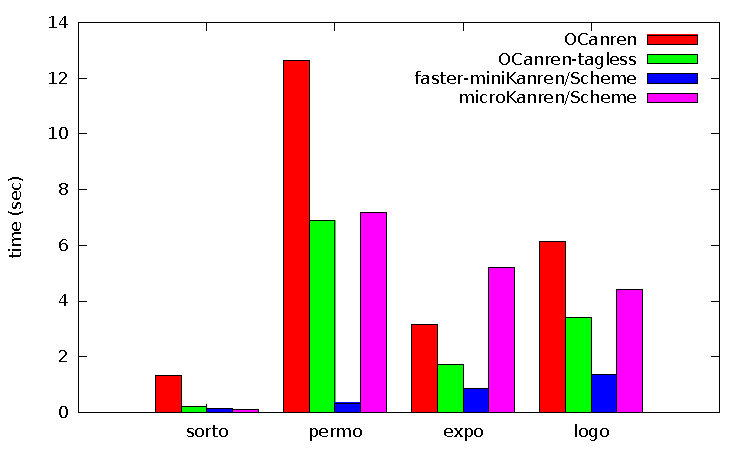
\includegraphics{graph1.pdf}
\caption{The First Set of Benchmarks}
\label{eval:first}
\end{figure}

\begin{figure}[h]
\centering
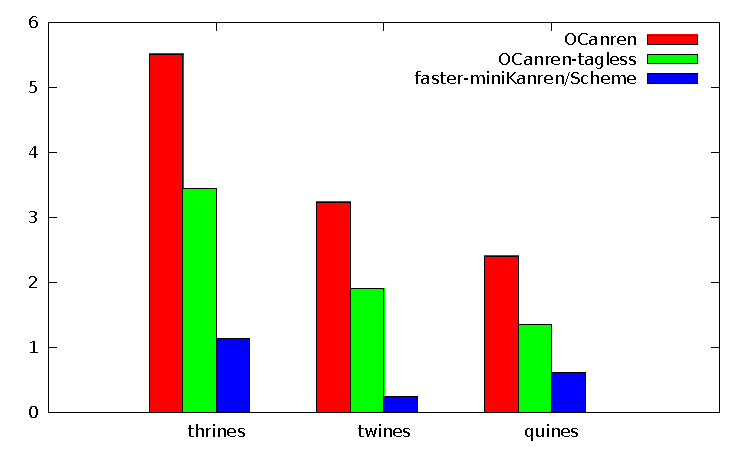
\includegraphics{graph2.pdf}
\caption{The Second Set of Benchmarks}
\label{eval:second}
\end{figure}

\section{Conclusion}

We presented a strongly-typed implementation of \miniKanren for OCaml. Our implementation
passes all tests written for \miniKanren (including those for disequality constraints);
in addition we implemented many interesting relational programs known from
the literature. We claim that our implementation can be used both as a convenient
relational DSL for OCaml and an experimental framework for future research in the area of
relational programming.

%We also want to express our gratitude to William Byrd, who infected us with relational programming,
%and for the extra time he sacrificed as both our tutor and friend.


\begin{comment}
\section{The Source Language}

\begin{figure}
\centering
{\bf Supplementary syntax categories:}
$$
\begin{array}{rcll}
  \mathcal C &=&\lstinline|True|,\,\lstinline|False|,\,C^n,\dots                &\mbox{\supp(constructors with arity)}\\
  \mathcal X &=&x,\,y,\,z,\,\dots                                               &\mbox{\supp(variables)}\\
  \mathcal P &=&C^n\,(x_1,\,\dots,\,x_n)                                         &\mbox{\supp(shallow patterns)}
\end{array}
$$
{\bf Expressions:}
$$
\begin{array}{rcll}
  \mathcal E &=&x                                                               &\mbox{\supp(variable occurrence)}\\
             & &\lambda x.e                                                     &\mbox{\supp(abstraction)}\\
             & &e_1\;e_2                                                        &\mbox{\supp(application)}\\ 
             & &C^n(e_1,\dots, e_n)                                             &\mbox{\supp(constructor application)}\\
             & &\lstinline|let $x$ = $e_1$ in $e_2$|                            &\mbox{\supp(let-binding)}\\
             & &\lstinline|let rec $f$ = $\lambda x.e_1$ in $e_2$|              &\mbox{\supp(recursive let-binding)}\\
             & &e_1\,=\,e_2                                                     &\mbox{\supp(equality test)}\\
             & &\lstinline|match $e$ with $\{p_i$ -> $e_i\}$| &\mbox{\supp(pattern matching)}
\end{array}
$$
\caption{Syntax of the source language}
\label{functional_syntax}
\end{figure}

\setarrow{:}
\newcommand{\typed}[3]{\withenv{#1}{\trans{#2}{}{#3}}}

\begin{figure}
\centering
{\bf Types:}
$$
\begin{array}{rcll}
  \mathcal X &=&\alpha, \beta, \dots                                            &\mbox{\supp{(type variables)}}\\
  \mathcal D &=&T^n,...                                                         &\mbox{\supp{(datatype constructors)}}\\
  \mathcal T &=&\lstinline|bool|\mid\alpha\mid T^n(t_1,\dots,t_n)\mid t_1\to t_2 &\mbox{\supp{(types)}}\\
  \mathcal S &=&\forall\bar{\alpha}.t                                           &\mbox{\supp{(type schemas)}}
\end{array}
$$
{\bf Typing rules:}
\begin{tabular}{p{7cm}p{7cm}}
$$
\typed{\Gamma}{\lstinline|True|,\;\lstinline|False|}{\lstinline|bool|}
\ruleno{Bool$_T$}
$$ 
&
$$
\trule{\typed{\Gamma}{e_1}{t}\;\;\;\;\typed{\Gamma}{e_2}{t}}
      {\typed{\Gamma}{e_1=e_2}{\lstinline|bool|}}
\ruleno{Eq$_T$}
$$
\\
$$
\trule{\typed{\Gamma}{e_i}{t^C_i}}
      {\typed{\Gamma}{C^n(e_1,\dots,e_n)}{t^C}}
\ruleno{Constr$_T$}
$$
&
$$
\typed{\Gamma,x:\forall\bar{\alpha}.t}{x}{t[\bar{\alpha}\gets\bar{t^\prime}]}
\ruleno{Var$_T$}
$$
\\
$$
\trule{\typed{\Gamma}{f}{t_1\to t_2}\;\;\;\;\typed{\Gamma}{e}{t_1}}
      {\typed{\Gamma}{f\;e}{t_2}}
\ruleno{App$_T$}
$$
&
$$
\trule{\typed{\Gamma,\,x:t_1}{f}{t_2}}
      {\typed{\Gamma}{\lambda x.f}{t_1\to t_2}}
\ruleno{Abs$_T$}
$$
\\
\multicolumn{2}{p{14cm}}{
$$
\trule{\typed{\Gamma}{e_1}{t_1}\;\;\;\;\typed{\Gamma,x:\forall\bar{\alpha}.t_1}{e_2}{t}}
      {\typed{\Gamma}{\lstinline|let $\;x\;$ = $\;e_1\;$ in $\;e_2$|}{t}},\;\bar{\alpha}=FV(t_1)\setminus FV(\Gamma)
\ruleno{Let$_T$}
$$}\\
\multicolumn{2}{p{14cm}}{
$$
\trule{\typed{\Gamma,f:t_1}{\lambda x.e_1}{t_1}\;\;\;\;\typed{\Gamma,f:\forall\bar{\alpha}.t_1}{e_2}{t}}
      {\typed{\Gamma}{\lstinline|let rec $\;f\;$ = $\;\lambda x.e_1\;$ in $\;e_2$|}{t}},\;\bar{\alpha}=FV(t_1)\setminus FV(\Gamma)
\ruleno{LetRec$_T$}
$$}\\
\multicolumn{2}{p{14cm}}{
$$
\trule{\typed{\Gamma}{e}{t^C}\;\;\;\;\typed{\Gamma,x^i_1:t^{C_i}_1,\dots,x^i_{k_i}:t^{C_i}_{k_i}}{e_i}{t}}
      {\typed{\Gamma}{\lstinline|match $\;e\;$ with $\;\{C_i^{k_i}(x^i_1,\dots,x^i_{k_i})$ -> $e_i\}$|}{t}}
\ruleno{Match$_T$}
$$}
\end{tabular}
\caption{Typing rules for the source language}
\label{functional_typing}
\end{figure}

\setarrow{\to}
\newcommand{\step}[2]{\trans{\inbr{#1}}{}{\inbr{#2}}}

\begin{figure}
\centering
{\bf Values:}
$$
\mathcal V = \lstinline|True|\mid\lstinline|False|\mid C^n(v_1,\dots,v_n)\mid\lambda x.e\mid\mu f\lambda x.e
$$
{\bf Contexts:}
$$
\mathcal C = \Box\;e\mid v\;\Box\mid\lstinline|let $x$ = $\Box$ in $e$|\mid\lstinline|match $\;\Box\;$ with $\{p_i$->$e_i\}$|\mid C^n(\bar{v},\Box,\bar{e})\mid\Box=e\mid v=\Box 
$$
$$
C[e]\mbox{\supp{~--- a context $C$ with an expression $e$ plugged into a hole}}
$$
{\bf Stack of contexts:}
$$
\mathcal S=\epsilon\mid\mathcal C : \mathcal S
$$
{\bf States:}
$$
\inbr{\mathcal S, e}\mbox{\supp{(stack of contexts, expression)}};\;\inbr{\epsilon,e}\mbox{\supp{(initial state)}};\;\inbr{\epsilon,v}\mbox{\supp{(final state)}}
$$
{\bf Transitions:}
\vskip2mm
\bgroup
\def\arraystretch{0}
\begin{tabular}{p{7cm}p{7cm}}
\multicolumn{2}{p{14cm}}{
$$
\step{C:\mathcal S,\, v}{\mathcal S,\, C[v]}\ruleno{Value}
$$}\\
$$
\step{\mathcal S,\, f\;e}{\Box\;e:\mathcal S,\, f}\ruleno{AppL}
$$&
$$
\step{\mathcal S,\, v\;e_2}{v\;\Box:\mathcal S,\, e_2}\ruleno{AppR}
$$\\
$$
\step{\mathcal S,\,e_1=e_2}{\Box=e_2:\mathcal S,\,e_1}\ruleno{EqL}
$$&
$$
\step{\mathcal S,\,v=e}{v=\Box:\mathcal S,\,e}\ruleno{EqR}
$$\\
\multicolumn{2}{p{14cm}}{
$$
\step{C:\mathcal S,\,v=v}{\mathcal S,\,C[\lstinline|True|]}\ruleno{EqTrue}
$$}\\
\multicolumn{2}{p{14cm}}{
$$
\step{C:\mathcal S,\,v_1=v_2}{\mathcal S,\,C[\lstinline|False|]},\;v_1\ne v_2\ruleno{EqFalse}
$$}\\
\multicolumn{2}{p{14cm}}{
$$
\step{\mathcal S,\, (\lambda x.e)\;v}{\mathcal S,\, e[x\gets v]}\ruleno{Beta}
$$}\\
\multicolumn{2}{p{14cm}}{
$$
\step{\mathcal S,\, (\mu f\lambda x.e)\;v}{\mathcal S,\, e[f\gets\mu f\lambda x.e,\, x\gets v]}\ruleno{Mu}
$$}\\
\multicolumn{2}{p{14cm}}{
$$
\step{\mathcal S,\, C^n(v_1,\dots,v_{k-1},e_k,\dots,e_n)}{C^n(v_1,\dots,v_{k-1},\Box,\dots,e_n):\mathcal S,\, e_k}\ruleno{Constr}
$$}\\
\multicolumn{2}{p{14cm}}{
$$
\step{\mathcal S,\, \lstinline|let $\;x\;$ = $\;e_1\;$ in $\;e_2$|}{\lstinline|let $\;x\;$ = $\;\Box\;$ in $\;e_2$|:\mathcal S,\, e_1}\ruleno{Let}
$$}\\
\multicolumn{2}{p{14cm}}{
$$
\step{\mathcal S,\, \lstinline|let $\;x\;$ = $\;v\;$ in $\;e$|}{\mathcal S,\,e[x\gets v]}\ruleno{LetVal}
$$}\\
\multicolumn{2}{p{14cm}}{
$$
\step{\mathcal S,\, \lstinline|let rec $\;f\;$ = $\;\lambda x.e_1\;$ in $\;e_2$|}{\mathcal S,\, e_2[f\gets\mu f\lambda x.e_1]}\ruleno{LetRec}
$$}\\
\multicolumn{2}{p{14cm}}{
$$
\step{\mathcal S,\,\lstinline|match $\;e\;$ with $\;\{p_i$->$e_i\}$|}{\lstinline|match $\;\Box\;$ with $\;\{p_i$->$e_i\}$|:\mathcal S,\, e}\ruleno{Match}
$$}\\
\multicolumn{2}{p{14cm}}{
$$
\step{\mathcal S,\,\lstinline|match $\;C_k^{n_k}(v_1,\dots,v_{n_k})\;$ with $\;\{C_i^{n_i}(x^i_1,\dots,x^i_{n_i})\to e_i\}$|}{\mathcal S,\,e_k[x^k_j\gets v_j]}\ruleno{MatchVal}
$$}
\end{tabular}
\egroup
\caption{Semantics for the source language}
\label{functional_semantics}
\end{figure}

\begin{figure}
\centering
$$
\begin{array}{rcll}
  \mathcal E &\mathrel{{+}{=}}&\lstinline|fresh ($x$) $\;e$| &\mbox{\supp{(fresh logical variable binder)}}\\
             &                &e_1\equiv e_2                 &\mbox{\supp{(unification)}}                   \\
             &                &e_1\not\equiv e_2             &\mbox{\supp{(disequality constraint)}}        \\
             &                &e_1\vee e_2                   &\mbox{\supp{(disjunction)}}                   \\
             &                &e_1\wedge e_2                 &\mbox{\supp{(conjunction)}}
\end{array}
$$
\caption{Syntax of the relational extension}
\label{relational_syntax}
\end{figure}

\setarrow{:}
\begin{figure}
\centering
{\bf Types:}
$$
\begin{array}{rcll}
 \mathcal L &=               &\;\uparrow\!\alpha \mid\;\uparrow\!\lstinline|bool|\mid\;\uparrow\!T^n(l_1,\dots,l_n)&\mbox{\supp{(type of logical terms)}}\\
 \mathcal T &\mathrel{{+}{=}}& \G                                                                            &\mbox{\supp{(type of logical goals)}}
\end{array}
$$
{\bf Typing rules:}
\begin{tabular}{p{7cm}p{7cm}}
\multicolumn{2}{p{14cm}}{
$$
\trule{\typed{\Gamma,x:l}{e}{\G}}
      {\typed{\Gamma}{\lstinline|fresh ($x$) $\;e$|}{\G}}
\ruleno{Fresh$_T$}
$$}\\
$$
\trule{\typed{\Gamma}{e_1}{l}\;\;\;\;\typed{\Gamma}{e_2}{l}}
      {\typed{\Gamma}{e_1\equiv e_2}{\G}}
\ruleno{Unify$_T$}
$$&
$$
\trule{\typed{\Gamma}{e_1}{l}\;\;\;\;\typed{\Gamma}{e_2}{l}}
      {\typed{\Gamma}{e_1\not\equiv e_2}{\G}}
\ruleno{Disequality$_T$}
$$\\
$$
\trule{\typed{\Gamma}{e_1}{\G}\;\;\;\;\typed{\Gamma}{e_2}{\G}}
      {\typed{\Gamma}{e_1\wedge e_2}{\G}}
\ruleno{Conjunction$_T$}
$$&
$$
\trule{\typed{\Gamma}{e_1}{\G}\;\;\;\;\typed{\Gamma}{e_2}{\G}}
      {\typed{\Gamma}{e_1\vee e_2}{\G}}
\ruleno{Disjunction$_T$}
$$
\end{tabular}
\caption{Typing rules for the relational extension}
\label{relational_typing}
\end{figure}

\setarrow{\to}
\begin{figure}
\centering
{\bf Semantic variables:}
\begin{gather*}
\mathfrak S = \mathfrak s_1, \mathfrak s_2, \dots\\
\Sigma, \Sigma^\prime\dots \subset 2^{\mathcal S}\;\mbox{\supp{(sets of allocated semantics variables)}}\\
\inbr{\Sigma^\prime, \mathfrak s}\gets\lstinline|new|\;\Sigma,\;\Sigma^\prime=\Sigma\cup\{\mathfrak s\}\;\mbox{\supp{(allocation of a new semantic variable)}}
\end{gather*}
{\bf Values:}
$$
\mathcal V \mathrel{{+}{=}} \lstinline|success|\mid\mathfrak s
$$
{\bf Contexts:}
$$
\mathcal C \mathrel{{+}{=}}\Box\equiv e\mid v\equiv\Box\mid\Box\not\equiv e\mid v\not\equiv\Box\mid\Box\wedge e\mid e\wedge\Box
$$
{\bf States:}
\begin{gather*}
\inbr{\Sigma,\mathcal S,e,\sigma}\mbox{\supp{(set of allocated semantic variables, stack of contexts, expression, logical state)}}\\
\inbr{\emptyset,\epsilon,e,\iota}\mbox{\supp{(initial state)}}\\
\inbr{\_,\epsilon,\lstinline|success|,\sigma}\mbox{\supp{(final state)}}
\end{gather*}
{\bf Transitions:}
\vskip2mm
\bgroup
\def\arraystretch{0}
\begin{tabular}{p{14cm}}
$$
\step{\Sigma,\,\mathcal S,\,\lstinline|fresh($x$) $\;e$|,\,\sigma}{\Sigma^\prime,\,\mathcal S,\,e[x\gets\mathfrak s],\,\sigma},\,\inbr{\Sigma^\prime,\mathfrak s}\gets\lstinline|new|\;\Sigma\ruleno{Fresh}
$$\\
$$
\step{\Sigma,\,\mathcal S,\,e_1\equiv e_2,\,\sigma}{\Sigma,\,\Box\equiv e_2:\mathcal S,\,e_1,\,\sigma}\ruleno{UnifyL}
$$\\
$$
\step{\Sigma,\,\mathcal S,\,v\equiv e,\,\sigma}{\Sigma,\,v\equiv\Box:\mathcal S,\,e,\,\sigma}\ruleno{UnifyR}
$$\\
$$
\step{\Sigma,\,\mathcal S,\,v_1\equiv v_2,\,\sigma}{\Sigma,\,\mathcal S,\,\lstinline|success|,\,\sigma^\prime},\,{\bf unify}\,(\sigma,\,v_1,\,v_2)=\sigma^\prime\ruleno{Unify}
$$\\
$$
\step{\Sigma,\,\mathcal S,\,e_1\not\equiv e_2,\,\sigma}{\Sigma,\,\Box\not\equiv e_2:\mathcal S,\,e_1,\,\sigma}\ruleno{DisEqL}
$$\\
$$
\step{\Sigma,\,\mathcal S,\,v\not\equiv e,\,\sigma}{\Sigma,\,v\not\equiv\Box:\mathcal S,\,e,\,\sigma}\ruleno{DisEqR}
$$\\
$$
\step{\Sigma,\,\mathcal S,\,v_1\not\equiv v_2,\,\sigma}{\Sigma,\,\mathcal S,\,\lstinline|success|,\,\sigma^\prime},\,{\bf diseq}\,(\sigma,\,v_1,\,v_2)=\sigma^\prime\ruleno{DisEq}
$$\\
$$
\step{\Sigma,\,\mathcal S,\,e_1\vee e_2,\,\sigma}{\Sigma,\,\mathcal S,\,e_1,\,\sigma}\ruleno{DisjL}
$$\\
$$
\step{\Sigma,\,\mathcal S,\,e_1\vee e_2,\,\sigma}{\Sigma,\,\mathcal S,\,e_2,\,\sigma}\ruleno{DisjR}
$$\\
$$
\step{\Sigma,\,\mathcal S,\,e_1\wedge e_2,\,\sigma}{\Sigma,\,\Box\wedge e_2:\mathcal S,\,e_1,\,\sigma}\ruleno{ConjStartL}
$$\\
$$
\step{\Sigma,\,\mathcal S,\,e_1\wedge e_2,\,\sigma}{\Sigma,\,e_1\wedge\Box:\mathcal S,\,e_2,\,\sigma}\ruleno{ConjStartR}
$$\\
$$
\step{\Sigma,\,\mathcal S,\,\lstinline|success|\wedge e,\,\sigma}{\Sigma,\,\mathcal S,\,e,\,\sigma}\ruleno{ConjL}
$$\\
$$
\step{\Sigma,\,\mathcal S,\,e\wedge\lstinline|success|,\,\sigma}{\Sigma,\,\mathcal S,\,e,\,\sigma}\ruleno{ConjR}
$$
\end{tabular}
\egroup
\caption{Semantics for the relational extension}
\label{relational_semantics}
\end{figure}

\begin{figure}
\centering
{\bf Terms:}
$$
\mathfrak T = \mathfrak s\mid\;\uparrow\!C^n(\mathfrak t_1,\dots,\mathfrak t_n)
$$
{\bf Substitution:}
\begin{gather*}
\theta:\mathfrak S\to\mathfrak T\;\mbox{\supp{(a partial mapping from semantic variables to terms)}}\\
\forall\theta\;\forall\mathfrak s,\mathfrak s^\prime\in dom(\theta)\;:\;\theta(\mathfrak s)\not\ni\mathfrak s^\prime\\
\mbox{\supp{Substitution application:}}\;\mathfrak t\theta=\left\{\begin{array}{rcl}
                           \theta\;\mathfrak s&,&\mathfrak s\in dom(\theta)\\
                           \uparrow\!C^n(\mathfrak t_1\theta,\dots,\mathfrak t_n\theta)&,&\mathfrak t=\uparrow\!C^n(\mathfrak t_1,\dots,\mathfrak t_n)\\
                           \mathfrak t&,&\mbox{\supp{otherwise}}
                         \end{array}
                  \right.\\
\phi\;\theta=\lambda\mathfrak s\,.\,(\theta\;\mathfrak s)\phi\;\mbox{\supp{(substitution composition)}}
\end{gather*}
{\bf Logical state:}
$$
\sigma=\inbr{\theta, \{\zeta_1,\dots,\zeta_k\}}\;\mbox{\supp{(a pair of a substitution and a set of substitutions)}}
$$
{\bf Unification:}
$$
{\bf unify}\,(\inbr{\theta, \{\zeta_1,\dots,\zeta_k\}}, \mathfrak t_1,\mathfrak t_2)
$$
{\bf Disequality constraint:}
$$
{\bf diseq}\,(\inbr{\theta, \{\zeta_1,\dots,\zeta_k\}}, \mathfrak t_1,\mathfrak t_2)
$$
\caption{Logical states and transitions}
\end{figure}
%\end{comment}

\begin{figure}
\centering
{\bf Ground types:}
$$
\mathcal G=\alpha\mid\lstinline|bool|\mid T^n(g_1,\dots,g_n)
$$
{\bf Type conversion:}
$$
\begin{array}{rcl}
\left[g\right]              &=&g\to\G\\
\left[t_1\to t_2\right]     &=&\left[t_1\right]\to\left[t_2\right]\\
\left[\forall\alpha.t\right]&=&\forall\alpha.\left[t\right]
\end{array}
$$
{\bf Term conversion:}
\vskip2mm
\bgroup
\def\arraystretch{0.2}
\begin{tabular}{p{7cm}p{7cm}}
\multicolumn{2}{p{14cm}}{$$
\sembr{x} = x\ruleno{Var$_{RC}$}
$$}\\
$$
\sembr{\lambda x.e}=\lambda x.\sembr{e}\ruleno{Abs$_{RC}$}
$$&
$$
\trule{e : \_\to\_}
      {\sembr{f\;e}=\sembr{f}\;\sembr{e}}\ruleno{App$_{RC}$}
$$\\
$$
\sembr{\lstinline|True|}=\lambda q\,.\,q\;\equiv\;\uparrow\!\lstinline|True|\ruleno{True$_{RC}$}
$$&
$$
\sembr{\lstinline|False|}=\lambda q\,.\,q\;\equiv\;\uparrow\!\lstinline|False|\ruleno{False$_{RC}$}
$$\\
\multicolumn{2}{p{14cm}}{$$
\sembr{\lstinline|let $\;x\;$ = $\;e_1\;$ in $\;e_2$|}=\lstinline|let $\;x\;$ = $\;\sembr{e_1}\;$ in $\;\sembr{e_2}$|\ruleno{Let$_{RC}$}
$$}\\
\multicolumn{2}{p{14cm}}{$$
\sembr{\lstinline|let rec $\;f\;$ = $\;e_1\;$ in $\;e_2$|}=\lstinline|let rec $\;f\;$ = $\;\sembr{e_1}\;$ in $\;\sembr{e_2}$|\ruleno{LetRec$_{RC}$}
$$}\\
\multicolumn{2}{p{14cm}}{$$
\trule{e : g\;\;\;\;f : g\to t_1\to\dots\to t_n\to g_0}
      {\sembr{f\;e}=\lambda y_1\dots y_nq\,.\,\lstinline|fresh ($q^\prime$) $\;(\sembr{e}\;q^\prime)\wedge(\sembr{f}\,(\equiv q^\prime)\,y_1\dots y_n\,q)$|}\ruleno{AppG$_{RC}$}
$$}\\
\multicolumn{2}{p{14cm}}{$$
\sembr{C^n(x_1,\dots,x_n)}=\lambda q\,.\,\lstinline|fresh ($q_1\dots q_n$)|\;(\bigwedge\sembr{x_i}\;q_i)\wedge(q\;\equiv\;\uparrow\!C^n(q_1,\dots,q_n))\ruleno{Constr$_{RC}$}
$$}\\
\multicolumn{2}{p{14cm}}{$$
\trule{\lstinline|match $\;e\;$ with $\;\{C^{n_i}_i(x^i_1,\dots,x^i_{n_i})\;$->$e_i\}$|:t_1\to\dots\to t_r\to g}
      {
       \begin{array}{ccc}
                        \multicolumn{3}{l}{\sembr{\lstinline|match $\;e\;$ with $\;\{C^{n_i}_i(x^i_1,\dots,x^i_{n_i})\;$->$e_i\}$|}=}\\ 
            \phantom{X}&\multicolumn{2}{l}{
                           \begin{array}{l}
                              \lambda q_1\dots q_rq\,.\,\lstinline|fresh ($s$)|\\
                              \phantom{XX}(\sembr{e}\;s)\wedge\\
                              \phantom{XX}\bigvee\lstinline|fresh ($s^i_1\dots s^i_{n_i}$)|\\
                              \phantom{XXXX}(s\;\equiv\;\uparrow\!C^{n_i}_i(s^i_1,\dots,s^i_{n_i}))\wedge\\
                              \phantom{XXXX}(\lambda x^i_1,\dots,x^i_{n_i}\,.\,\sembr{e_i}\;q_1\dots q_r\;q)(\equiv\;s^i_1)\dots(\equiv\;s^i_{n_i})
                           \end{array}}                        
       \end{array}
      }\ruleno{Match$_{RC}$}
$$}\\
\multicolumn{2}{p{14cm}}{$$
\begin{array}{ccc}
                \multicolumn{3}{l}{\sembr{e_1=e_2}=}\\
    \phantom{X}&\multicolumn{2}{l}{
       \begin{array}{l}
        \lambda q\,.\,\lstinline|fresh ($q_1\;q_2$)|\\
        \phantom{XX}(\sembr{e_1}\;q_1)\wedge\\
        \phantom{XX}(\sembr{e_2}\;q_2)\wedge\\
        \phantom{XX}((q_1\;\equiv\;q_2\wedge q\;\equiv\;\uparrow\!\lstinline|True|)\vee(q_1\;\not\equiv\;q_2\wedge q\;\equiv\;\uparrow\!\lstinline|False|))
       \end{array}
    }
\end{array}\ruleno{Eq$_{RC}$}
$$}
\end{tabular}
\egroup
\caption{Relational conversion rules}
\end{figure}
\end{comment}

\printbibliography

\begin{comment}
\begin{thebibliography}{99}
\bibitem{TRS}
Daniel P. Friedman, William E.Byrd, Oleg Kiselyov. The Reasoned Schemer. The MIT
Press, 2005.

\bibitem{MicroKanren}
Jason Hemann, Daniel P. Friedman. $\mu$Kanren: A Minimal Core for Relational Programming //
Proceedings of the 2013 Workshop on Scheme and Functional Programming (Scheme '13).

\bibitem{alphaKanren}
William E. Byrd, Daniel P. Friedman. alphaKanren: A Fresh Name in Nominal Logic Programming //
Proceedings of the 2007 Workshop on Scheme and Functional Programming (Scheme '07).

\bibitem{CKanren}
Claire E. Alvis, Jeremiah J. Willcock, Kyle M. Carter, William E. Byrd, Daniel P. Friedman.
cKanren: miniKanren with Constraints //
Proceedings of the 2011 Workshop on Scheme and Functional Programming (Scheme '11).

\bibitem{Untagged}
William E. Byrd, Eric Holk, Daniel P. Friedman.
miniKanren, Live and Untagged: Quine Generation via Relational Interpreters (Programming Pearl) //
Proceedings of the 2012 Workshop on Scheme and Functional Programming (Scheme '12).

%\bibitem{Implicits}
%Leo White, Fr\'ed\'eric Bour, Jeremy Yallop.
%Modular Implicits // Workshop on ML, 2014, arXiv:1512.01438.

%\bibitem{Unparsing}
%Olivier Danvy.
%Functional Unparsing // Journal of Functional Programming, Vol.~8, Issue~6, November 1998.

%\bibitem{DoWeNeed}
%Daniel Fridlender, Mia Indrika.
%Do we need dependent types? // Journal of Functional Programming, Vol.~10, Issue~4, July 2000.

%\bibitem{DGP}
%Jeremy Gibbons. Datatype-generic Programming //
%Proceedings of the 2006 International Conference on Datatype-generic Programming.

%\bibitem{Deriving}
%Jeremy Yallop.
%Practical Generic Programming in OCaml // Proceedings of 2007 Workshop on ML.

%\bibitem{InstantGenerics}
%Manuel M. T. Chakravarty, Gabriel C. Ditu, Roman Leshchinskiy.
%Instant Generics: Fast and Easy. \url{http://www.cse.unsw.edu.au/~chak/papers/CDL09.html}, 2009.

%\bibitem{ALaCarte}
%Wouter Swierstra. Data Types \'a la Carte  // Journal of Functional Programming, Vol.~18, Issue~4, 2008.

%\bibitem{Kumar}
%Ramana Kumar. Mechanising Aspects of miniKanren in HOL. Bachelor Thesis, The Australian National University, 2010.

\bibitem{Unification}
Franz Baader, Wayne Snyder. Unification theory. In John Alan Robinsonand Andrei Voronkov, editors,
Handbook of Automated Reasoning. Elsevier and MIT Press, 2001.

%\bibitem{triangular}
%David C Bender, Lindsey Kuper, William E Byrd, Daniel P Friedman.
%Efficient Representations for Triangular Substitutions: a Comparison in miniKanren. Indiana University, 2009.

%\bibitem{HKinded}
%Jeremy Yallop, Leo White. Lightweight Higher-Kinded Polymorphism. FLOPS 2014.

\bibitem{Lambda}
Henk Barendregt. Lambda Calculi with Types, Handbook of Logic in Computer Science (Vol.~2), 1992.

\bibitem{WillThesis}
William E. Byrd. Relational Programming in miniKanren: Techniques, Applications, and Implementations. PhD Thesis,
Indiana University, Bloomington, IN, September 30, 2009.

\bibitem{ocanren}
Dmitry Kosarev, Dmitry Boulytchev. Typed Embedding of a Relational Language in OCaml // International Workshop on ML, 2016.

\bibitem{Types}
Benjamin Pierce. Types and Programming Languages. MIT Press, 2002.

\bibitem{Felleisen}
Andrew Wright, Matthias Felleisen. A Syntactic Approach to Type Soundness // Information and Computation, Vol.~115, No.~1, 1994.

\bibitem{cardelli}
Luca Cardelli, Peter Wegner. On Understanding Types, Data Abstraction, and Polymorphism // ACM Computing Surveys, Vol.~17, No.~4, 1985.

\bibitem{unified}
William E. Byrd, Michael Ballantyne, Gregory Rosenblatt, Matthew Might. A Unified Approach to Solving Seven Programming Problems // 
Proceedings of the International Conference on Functional Programming, 2017.

\bibitem{WillOnHM}
William E. Byrd. Personal communications.

\end{thebibliography}
\end{comment}

\end{document}

